% !Mode:: "TeX:UTF-8"
%!TEX program  = xelatex

%\documentclass{cumcmthesis}
\documentclass[withoutpreface,bwprint]{cumcmthesis} %去掉封面与编号页

\usepackage{ulem}
\usepackage{subfigure}	%用于排版多张图片
\usepackage{float}	%用于排版图片位置
\normalem \bibliographystyle{plain}	%引用样式,参考文献

\usepackage{url}
\title{板凳龙沿等距螺线行进模型}

\begin{document}

\maketitle
\begin{abstract}

板凳龙是中国传统民俗活动，有悠久的历史。对于板凳龙盘入盘出的一般过程，本文建立数学模型，解决盘龙时遇到的相关问题。

对于问题一，首先建立极坐标系，通过螺距计算得出等距螺线的方程；接着，根据弧长与时间的关系，积分得出各时刻龙头的位置；最后分别根据把手间距为定值和沿板凳方向速度相等两等值条件，得出相邻龙身位置和速度的递推关系，进而计算出每秒舞龙队的位置和速度。

问题二要求我们确定舞龙队最终停止的时刻，并给出此时舞龙队的位置和速度。我们采用可视化的方法，通过碰撞检测，确定出龙头与第八节龙身发生碰撞，同时得出碰撞发生的大致时间范围。最后使用二分法计算出发生碰撞的位置，进而计算出发生碰撞的时间为412.473838$s$。

问题三需要确定使龙头前把手能够盘入调头空间边界的最小螺距。先根据问题二的结论得到大致的螺距取值范围，再通过可视化的处理,考虑扩大调头区域半径，找到碰撞发生的临界条件。据此使用二分法可计算出$a$的值，进而计算出最小螺距为$44.98051434cm$。

问题四
建立几何模型，利用几何关系求得题目条件下调头区域内路径总长度一定。扩展问题一的模型，用相似的方法，通过分类讨论，可以得到相邻龙身位置和速度的关系，进而计算出每秒舞龙队的位置和速度。

问题五要求得出使整个过程中速度不超过2m/s的最大龙头速度，从问题四的模型中，可以得出当位置固定时龙头速度与龙身速度呈正比的结论。据此，仅需得出各龙身的最大速度，便可根据速度的比例关系得出龙头的最大速度。通过构造求龙身速度最大值的函数，采用二分法即可求得速度最大的时刻，以及最大速度。根据比例关系可解得龙头速度最大值为1.246266m/s。

最后，本文对模型的优缺点分别进行了评价并给出了改进方法。

\keywords{板凳龙\quad 等距螺线\quad  可视化\quad  碰撞检测\quad  二分查找\quad}

\end{abstract}

%目录
%\tableofcontents

%新的一页
%\newpage

\section{问题重述}

板凳龙由几十上百条板凳首尾相连，其中第一节为龙头，最后一节为龙尾，其中均为龙身。每节板凳上均有两个孔，相邻的两节板凳由穿过孔的把手连接。盘龙时，龙头在前领头，龙身和龙尾相随盘旋，整体呈圆盘状。在舞龙队能够自如地盘入和盘出的前提下，盘龙所需要的面积越小、行进速度越快，则观赏性越好。建立模型解决以下问题：

问题一：舞龙队沿着螺距为$55cm$的等距螺线顺时针盘入，把手中心均位于螺线上。龙头前把手的速度恒为$1m/s$。初始时，龙头位置为螺线第十六圈的A点处。需要给出每秒整个舞龙队的位置和速度。

问题二：舞龙队沿着问题一设定的螺线盘入，确定舞龙队不能再继续盘入即板凳之间不发生碰撞的最后时刻，并给出此时舞龙队的位置和速度。

问题三：从盘入到盘出，舞龙队将由顺时针盘入到逆时针盘出。其掉头空间为以螺线中心为圆心、直径为$9m$的圆形区域，确定最小螺距使得龙头前把手能够沿着相应的螺线盘入到掉头空间的边界。

问题四：盘出螺线与螺距为$1.7m$盘入螺线关于螺线中心成中心对称。舞龙队在问题三的掉头空间内完成掉头，掉头路径为两段圆弧相切连成的S形曲线，前一段圆弧半径为后一段的两倍，与盘入、出螺线均相切。求问是否能够调整圆弧，使得在保持各部分相切的前提下，掉头曲线变得更短？龙头前把手的速度保持为$1m/s$。以掉头开始时间为零时刻，给出$-100s$到$100s$每秒舞龙队的位置和速度。

问题五：舞龙队沿着问题四的路线前进，龙头速度保持不变，需要求解使得舞龙队各把手的速度不超过2m/s的龙头的最大速度，。

\section{问题分析}

\subsection{问题一的分析}

问题一中，舞龙队沿着等距螺线盘绕，我们需要得到每秒整个舞龙队的位置和速度。而整个舞龙队的位置与速度依赖于龙头的位置、速度与行进路径，故而先由等距螺线本身的性质列出微分方程，再求解出该等距螺线的方程。

在计算出螺线方程之后，便可依据弧长与时间的关系，采用积分的手段确定出各个时刻龙头所在的具体位置，基于把手之间的距离为一定值，可通过以前一把手为圆心，把手距离为半径做圆的方式做出辅助圆，该圆与螺线方程的交点即为下一把手的位置所在。

对于速度的求解沿用相同的思路，对于第$n$个龙身与第$n+1$个龙身，通过沿板凳速度相等这一关系以及余弦定理等数学工具，可得出相邻龙身之间速度的递推关系，由此可依次得出整个舞龙队的各个时刻的速度。

\subsection{问题二的分析}

问题二要求求解舞龙队不能再继续盘入的最终时刻，定性分析之后确定龙头将与龙身首先发生碰撞。

将问题一中的数据进行可视化，得出内圈与外圈之间角速度的差值较小，据此可确定龙身与第八节龙身发生碰撞，同时得到发生碰撞时间的大致范围。

在大致时间内，计算出龙头边缘所有点的坐标，并求出龙身两把手之间连线，使用二分法计算出龙头龙身将发生碰撞的位置，得到位置之后便可采用问题一的模型计算出发生碰撞的时间。

\subsection{问题三的分析}

问题三需要确定使龙头前把手能够盘入到调头空间的边界的最小螺距。由问题二的结论与板凳的宽度可知此问题螺距的大致范围。

接下来改进问题二的所建立的模型，固定龙头的初位置（即$r_{0} = 4.5m$），以a为变量进行可视化处理。

可视化处理之后，可通过扩大调头区域半径$R$的方式改进问题二中的模型，进而通过二分法逼近使得龙头在进入调头区域即发生碰撞的对应的$r$值，再利用问题一的模型计算出最小螺距。
\subsection{问题四的分析}
将题目所给板凳龙行进轨迹抽象成几何模型，通过几何关系，可以确定对于一个正确的轨迹，有两圆弧圆心间距离相等以及圆心连线平行，进而得出板凳龙在掉头区间内行进的轨迹长度恒定。

绘制出题目所给轨迹，对于一节龙身的后把手，先确定其位于哪一段曲线上，再利用问题一的方法，联立依次求解各个把手的位置。对于速度，则可求得轨迹各个点的切线，利用问题一的方法求得各把手速度。
\subsection{问题五的分析}
对于问题五，由问题四的模型可知，位置固定时，龙身速度与龙头速度呈正比例关系。由此只要得出速度最大的时刻的最大速度，便可根据比例关系得出龙头的最大速度。

观察问题四表格发现，板凳龙在掉头圆弧的过程中，板凳与轨迹切线的夹角比较大，使得前后速度差距较大。由此可得出最大速度的时刻的大致范围。

在该范围内，通过构造函数来求解t时刻的最大速度，并利用此函数对时间t进行二分逼近，得到最大的速度。根据速度比例关系便可得出龙头的最大速度。
\section{模型假设}

1.假设盘龙过程中板凳始终保持水平；

2.假设盘龙过程中不存在阻碍盘龙正常行进的任何外力；

3.假设盘龙场地地面平整；

4.假设盘龙过程中每个人都能根据前一个人速度改变而立刻改变速度；


\section{符号说明}
\begin{center}
\begin{tabular}{cc}
 \toprule[1.5pt]
 \makebox[0.3\textwidth][c]{符号}	&  \makebox[0.4\textwidth][c]{说明} \\
 \midrule[1pt]
 $ d $	    	& 螺距   \\ 
 $ r $	    & 点到极点距离  \\ 
 $ \theta $	    	& 极角 \\ 
 $v_{0}  $   &龙头速度  \\
 $r_{0}  $    &龙头起始位置\\
\bottomrule[1.5pt]
\end{tabular}
\end{center}

\section{模型的建立与求解}

\subsection{问题一模型的建立与求解}

在计算整个舞龙队的位置和速度之前，需要先根据螺距计算出等距螺线的方程，为保持形式的简洁，此处采用极坐标系表示该等距螺线的方程，
即：
$$r=\frac{d}{2\pi} \theta  $$
\noindent 其中$d$为等距螺线的螺距,考虑到后续方程的简洁性，全文将用$a$替代$\frac{d}{2\pi}$。

计算出螺线方程之后，便可对弧长进行积分，并通过弧长与时间的关系，得到如下关系式：
$$
\begin{cases}
    &s=v_{0}t \\
    &s=a\int_{\theta }^{32\pi } \sqrt{1+  \varphi ^{2} } \mathrm{d}\varphi 
\end{cases}
$$

由此可得出龙头距螺线距离$r$与与时间$t$之间的关系，即：
$$\frac{r}{2} \sqrt{r^{2} +a^{2} } +\frac{a^{2} }{2} \ln_{}{\frac{r+\sqrt{r^{2} +a^{2} } }{r_{0}   +\sqrt{r_{0}^{2} +a^{2} } } }=\frac{r_{0} }{2}\sqrt{r_{0}^{2} +a^{2} }-av_{0}t    $$
其r-t图像如下：
\begin{figure}[H]
	\label{jmzbx}
	\centering
	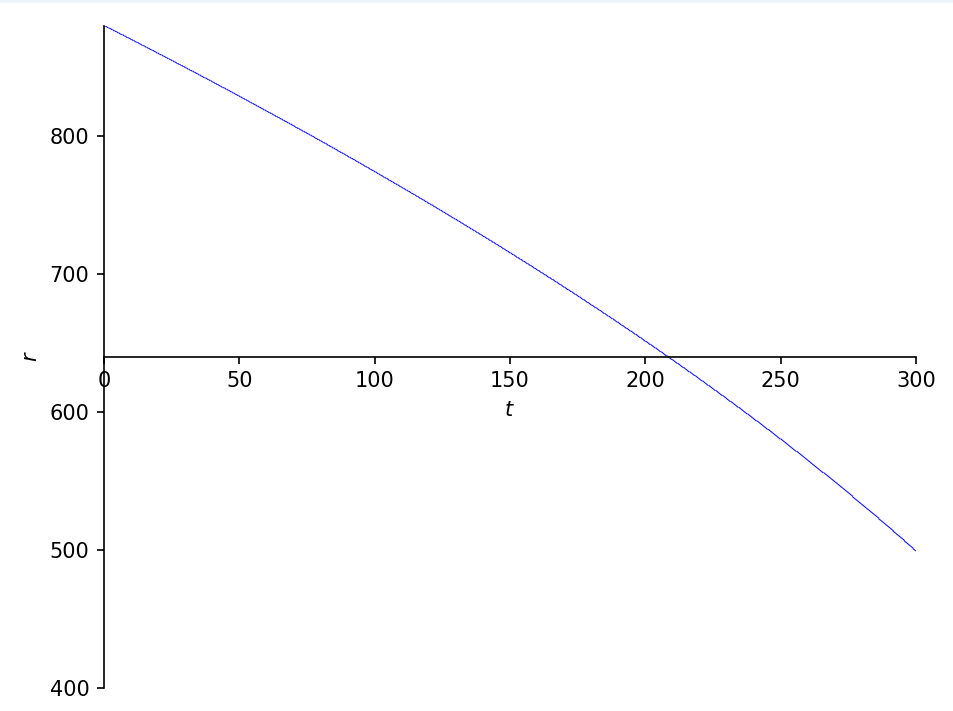
\includegraphics[width=12cm,height=12cm]{figures/r-t图像.png}	
	\caption{龙头前把手r-t图像}
\end{figure}

假设已知第n节龙身前把手的位置，则以该把手为圆心，第n节龙身与第n+1节龙身的把手之间距离为半径画出辅助圆，方程如下：
 $$l^{2}=\left ( r_{n+1}\cos\theta_{n+1}  - r_{n}\cos\theta_{n}\right  ) ^{2}+ \left ( r_{n+1}\sin\theta_{n+1}  - r_{n}\sin\theta_{n} \right ) ^{2}$$
 其中$l$表示龙头把手间的距离或龙身把手间距离，$r_{i}$、$\theta_{i}$表示第i节把手的极坐标。

\begin{figure}[H]
	\label{jmzbx}
	\centering
	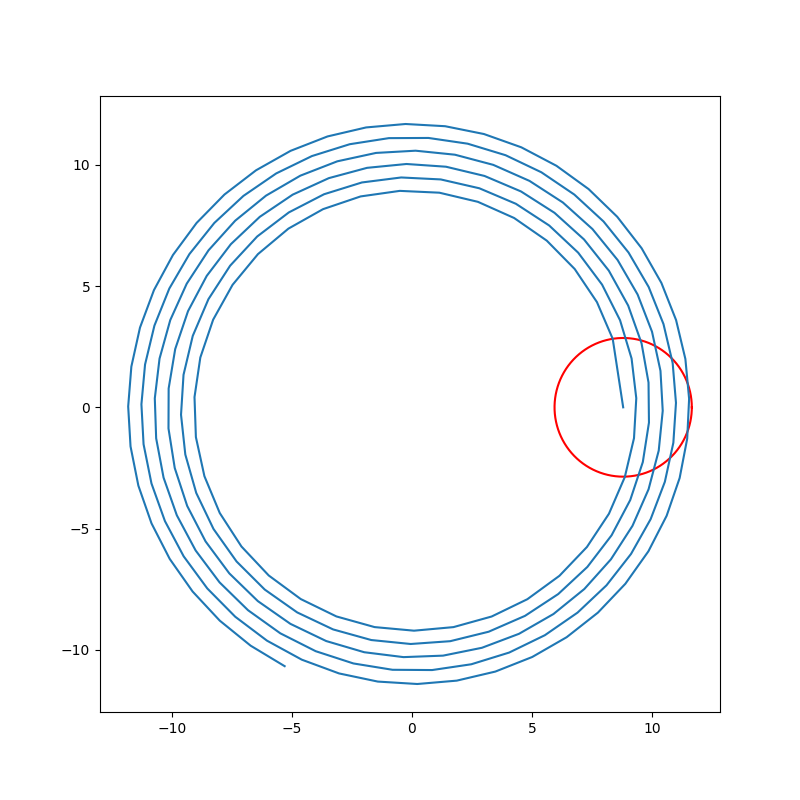
\includegraphics[width=8cm,height=8cm]{figures/位置求解示意.png}	
	\caption{位置求解示意}
\end{figure}

该圆与螺线的交点即为第n+1节龙身前把手的位置，多次联立可依次计算出舞龙队所在的位置，其在 0 s、60 s、120 s、180 s、240 s、300 s的位置如下表所示：
\begin{table}[H]
	\centering
	\caption{舞龙队各时刻位置}
	\begin{tabular}{|c|c|c|c|c|c|c|}
		\hline
		                 & 0 s     & 60 s     & 120 s   & 180 s  & 240 s  & 300 s     \\ \hline
龙头 x (m)         & 8.800000  & 5.799209  & -4.084887 & -2.963609 & 2.594494 &4.420274 \\ \hline
龙头 y (m)         & 0.000000  & -5.771092 & -6.304479 & 6.094780 & -5.356743&2.320429 \\ \hline
第 1 节龙身 x (m)   & 8.363824  & 7.456758 & -1.445473 & -5.237118 & 4.821221 & 2.459489\\ \hline
第 1 节龙身 y (m)   & 2.826544  & -3.440399 & -7.405883 & 4.359627 & -3.561949& 4.402476 \\ \hline
第 51 节龙身 x (m)  & -9.518732 & -8.686317 & -5.543150 &2.890455  & 5.980011 &-6.301346 \\ \hline
第 51 节龙身 y (m)  & 1.341137  & 2.540108 & 6.377946 & 7.249289   &-3.827758 & 0.465829 \\ \hline
第 101 节龙身 x (m) & 2.913983  & 5.687116 & 5.361939 &1.898794    &-4.917371 &-6.237722\\ \hline
第 101 节龙身 y (m) & -9.918311 & -8.001384 & -7.557638 & -8.471614 &-6.379874 & 3.936008 \\ \hline
第 151 节龙身 x (m) & 10.861726 & 6.682311 & 2.388757 &1.005154   & 2.965378& 7.040740 \\ \hline
第 151 节龙身 y (m) & 1.828753  & 8.134544 & 9.727411 & 9.424751  & 8.399721 & 4.393013 \\ \hline
第 201 节龙身 x (m) & 4.555102  & -6.619664 & -10.627211 &-9.287720 & -7.457151 &-7.458662 \\ \hline
第 201 节龙身 y (m) & 10.725118 & 9.025570 & 1.359847 &-4.246673  & -6.180726 & -5.263384 \\ \hline
龙尾（后） x (m)    & -5.305444 & 7.364557 & 10.974348 & 7.383896  & 3.241051 & 1.785033 \\ \hline
龙尾（后） y (m)    & -10.676584 & -8.797992 & 0.843473 & 7.492370 & 9.469336 & 9.301164\\ \hline
	\end{tabular}
\end{table}

速度求解过程如下：

\begin{figure}[H]
	\label{jmzbx}
	\centering
	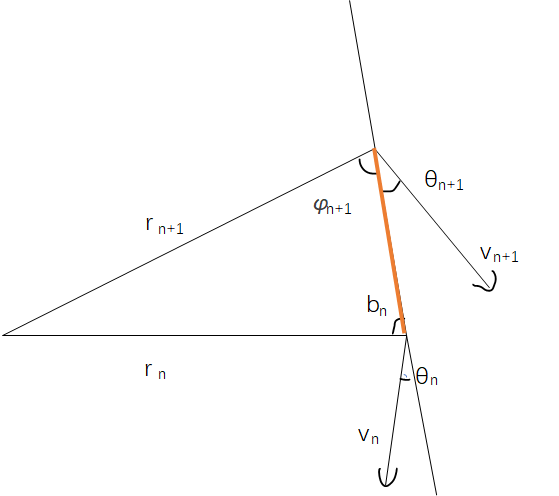
\includegraphics[width=10cm,height=7cm]{figures/速度求解示意.png}	
	\caption{速度求解示意}
\end{figure}
图中橙色部分为连接把手n与把手n+1的中间木板部分

由于沿板凳方向分速度相等，考察第n+1个点与第n个点的速度，有如下等式，式中各个变量名如图3：
$$v_{n+1} \times \cos (\theta _{n+1} )=v_{n} \times \cos (\theta _{n} )$$
速度方向延等距螺线切线方向，故可通过上文求得的位置信息，编程获得角度关系，从而依次求解后续点的速度大小，如下表所示
\begin{table}[H]
	\centering
	\caption{舞龙队各时刻速度}
	\begin{tabular}{|c|c|c|c|c|c|c|}
		\hline
           &0 s &60 s &120 s &180 s &240 s &300 s \\ \hline
龙头 (m/s) &1.0 &1.0 &1.0 &1.0 &1.0 &1.0\\ \hline
第1节龙身  (m/s) &0.999971 &0.999961 &0.999945 &0.999917 &0.999859 &0.999709 \\ \hline
第51节龙身  (m/s) &0.998750 &0.998367 &0.997777 &0.996796 &0.994981 &0.991007 \\ \hline
第101节龙身  (m/s) &0.996093 &0.994988 &0.993334 &0.990688 &0.986044 &0.976646 \\ \hline
第151节龙身  (m/s) &0.992518 &0.990539 &0.987639 &0.983130 &0.975507 &0.960851 \\ \hline
第201节龙身  (m/s) &0.988344 &0.985431 &0.981239 &0.974861 &0.964374 &0.944951 \\ \hline
龙尾（后） (m/s) &0.986372 &0.983044 &0.978285 &0.971105 &0.959417 &0.938061 \\ \hline
	\end{tabular}
\end{table}


\subsection{问题二模型的建立与求解}

将问题一中的数据进行可视化处理并加上矩形框表示板凳边缘，得到板凳龙的行进示意图如下：
\begin{figure}[H]
	\label{jmzbx}
	\centering
	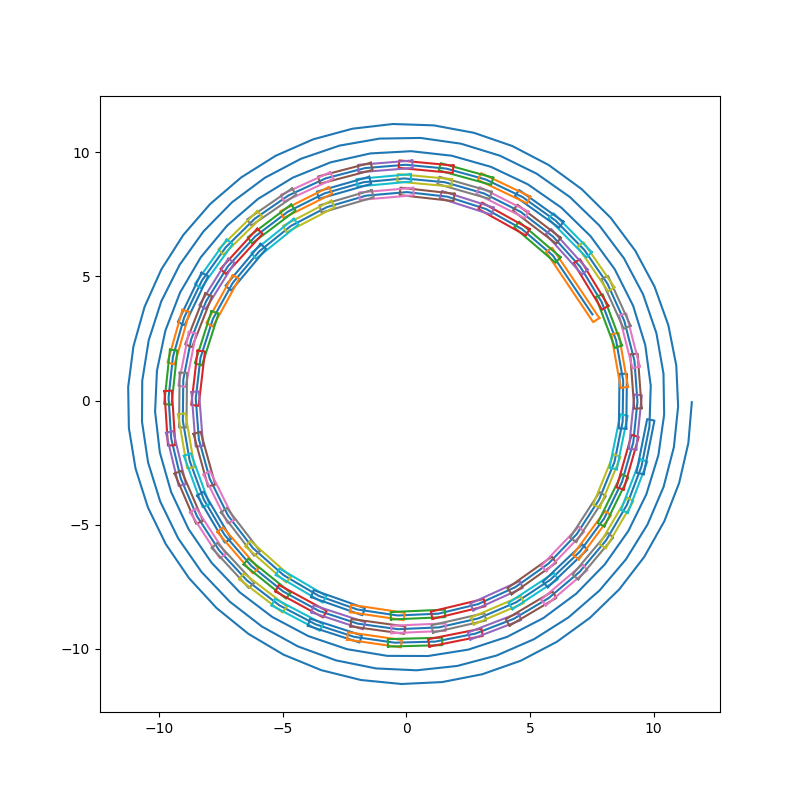
\includegraphics[width=12cm,height=12cm]{figures/板凳龙示意图.png}	
	\caption{板凳龙示意图}
\end{figure}

随着等距螺线上点与原点的距离减小，等距螺线的曲率逐渐增大，木板与螺线的拟合程度降低，与内侧一圈的螺线距离更近，故碰撞必然首先发生在内圈。同时由于龙头板凳长度更大，其木板边缘顶点距离龙头把手所在螺线距离更远。通过上述定性分析，可以初步判定，碰撞首先发生在龙头顶点处

若已知龙头前后把手坐标分别为$\left ( x_{d1},y_{d1} \right ) ,\left ( x_{d2},y_{d2} \right )$，龙身前后把手坐标分别为$\left ( x_{1},y_{1} \right ) ,\left ( x_{2},y_{2} \right )$,则可以建立如下碰撞检验模型：

龙身两把手之间连线方程为：
$$
\left ( y_{2}-y_{1}   \right ) x+\left ( x_{1}-x_{2}   \right ) y+\left ( x_{2}y_{1}-x_{1}y_{2}     \right )=0 
$$

龙头边缘点$\left ( x_{0},y_{0} \right )$的坐标方程满足
$$
\begin{cases}\tan \left ( \pi - \theta  \right ) =\frac{y_{d1}-y_{d2}}{x_{d1}-x_{d2}} \\x_{0}=x_{d1}+d_{w}\cos \theta +d_{l}\sin \theta  \\y_{0}=y_{d1}+d_{w}\sin \theta +d_{l}\cos \theta \end{cases}
$$
其中$d_{w}$为龙头前把手到宽边的距离，$d_{l}$为龙头前把手到长边的距离。

边缘点到把手连线的距离公式为：
$$
d_{e}=\frac{\left | \left ( y_{2}-y_{1}    \right )x_{0} +\left ( x_{1}-x_{2}   \right ) y_{0}+\left ( x_{2}y_{1}-x_{1}y_{2}     \right )    \right | }{\sqrt{\left ( y_{1}-y_{2}    \right )^{2}+\left ( x_{1}-x_{2}   \right ) ^{2}   } } 
$$
 当$d_{e}\le 15cm$时则龙头与龙身发生了碰撞。

通过计算板子相对于螺线中心的角速度，注意到内圈与外圈角速度相差极小，从而可以选取离散的若干时刻对板凳龙进行动态模拟。以步长为1s递增时间$t$模拟板凳龙行进的过程,经过碰撞检测得出与龙头首先发生碰撞的龙身为第八节，同时得到碰撞的时间区间为412.4$\sim $412.6$s$。在区间内用二分法得出碰撞时间的近似值$412.474s$，再使用问题一的模型可计算出该时刻整个舞龙队的位置和速度。

\begin{table}[H]
	\centering
	\caption{舞龙队最终时刻位置}
	\begin{tabular}{|c|c|c|}
		\hline
   &横坐标x (m)&纵坐标y (m)\\ \hline
龙头 &1.209930 &1.942784 \\ \hline
第1节龙身 &-1.643792 &1.753399 \\ \hline
第51节龙身 &1.281200 &4.326588 \\ \hline
第101节龙身 &-0.536246 &-5.880138 \\ \hline
第151节龙身 &0.968841 &-6.957479 \\ \hline
第201节龙身 &-7.893161 &-1.230764 \\ \hline
龙尾（后） &0.956216 &8.322736 \\ \hline
	\end{tabular}
\end{table}

\begin{table}[H]
	\centering
	\caption{舞龙队最终时刻速度}
	\begin{tabular}{|c|c|}
		\hline
  &速度 (m/s) \\ \hline
龙头 &1.0 \\ \hline
第1节龙身 &0.991551 \\ \hline
第51节龙身&0.921988 \\ \hline
第101节龙身 &0.860071 \\ \hline
第151节龙身 &0.809600 \\ \hline
第201节龙身 &0.767382 \\ \hline
龙尾（后） &0.750820 \\ \hline
	\end{tabular}
\end{table}

\subsection{问题三模型的建立与求解}

对于能盘入调头空间的最小螺距，注意到问题三所需螺距必定小于问题二所需螺距，且大于板凳宽度，判断出螺距$d$满足：
$$
30cm\le d\le 55cm
$$
对问题二的模型进行改进，固定龙头前把手的初位置于调头空间边缘（即$r_{0}=4.5m$），以$a$为变量进行可视化处理。

可视化处理后，注意到当a相近时，与龙头相对的次内圈龙身编号固定，则发生碰撞必定发生在龙头与此龙身之间，即第17节龙身.同时观察到两者前后把手连线斜率相近，说明已经完成碰撞。考虑到对于不同的a值，当调头区域半径固定时，在进入调头区域瞬间，龙头与外圈龙身的相对位置基本一致，由此可通过调整调头区域半径，来对所有a的情况进行调整，故调整半径至龙头进入调头区域时恰好发生碰撞，由此确定a的大致范围。此时，再联系问题一模型，进行考虑a与t双变量的碰撞检测，通过二分法求出a的相对精确的近似解

如此改进模型之后,计算得到最小螺距$d_{min}=44.98051434cm$



\subsection{问题四模型的建立与求解}

调整圆弧不能在保持相切的前提下缩短路径，而是路径总固定。建立如下几何模型给出证明：

\begin{figure}[H]
	\label{jmzbx}
	\centering
	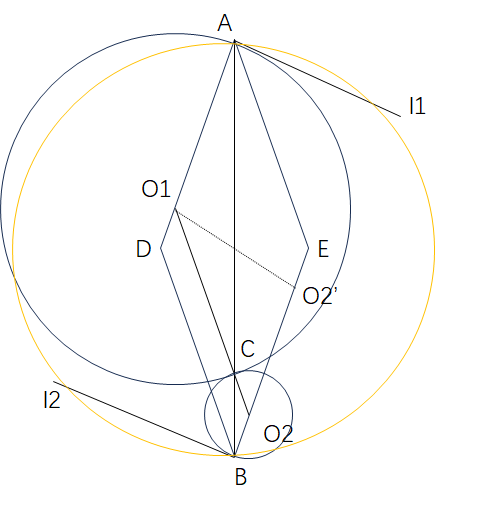
\includegraphics[width=12cm,height=12cm]{figures/q4几何模型.png}	
	\caption{问题四几何模型}
\end{figure}
设A点为盘入点，B点位盘出点，$l_{1},l_{2}$分别为盘入螺线与盘出螺线在盘入盘出点的切线，由于圆弧与螺线相切，故第一段圆弧圆心位于直线AD上，第二段圆弧圆心位于直线BE上，满足
$$AD\bot l_{1} ,BE\bot l_{2} $$
过A点作线段AE使得
$$\angle BAD=\angle BAE,AD=AE$$
进而建立菱形AEBD
不妨令圆心分别为$O_{1}$与$O_{2}$,$O_{1}O_{2}$与盘入盘出点连线$AB$交于点C。若$O_{1}O_{2}$//$AE$，则
$$O_{1}O_{2}=O_{1}C+O_{2}C=AO_{1}+BO_{2}$$
可见此时两圆符合题目要求；若$O_{1}O'_{2}$//$AE$不成立，则由题意有$O_{1}A+O'_{2}B=O_{1}O'_{2}$,但
$$O_{1}A+O'_{2}B=O_{1}A+BO_{2}+O'_{2}O_{2}=O_{1}O_{2}+O_{2}O'_{2}$$
$O_{1}O_{2}O'_{2}$构成三角形，满足
$$O_{1}O_{2}+O_{2}O'_{2}> O_{1}O'_{2}$$
与题意矛盾！所以有$O_{1}O_{2}$//$AE$，此时弧长$$s=\mid BO_{2} \mid \times \measuredangle BO_{2} C+\mid AO_{1} \mid \times \measuredangle AO_{1} C=AE\times \measuredangle AEB$$
可见弧长保持不变，即不能通过调整圆弧位置而缩小掉头的弧长。

由两院弧半径比为1：2，以及盘入盘出螺线中心对称，画出题目所给行进轨迹：
\begin{figure}[H]
	\label{jmzbx}
	\centering
	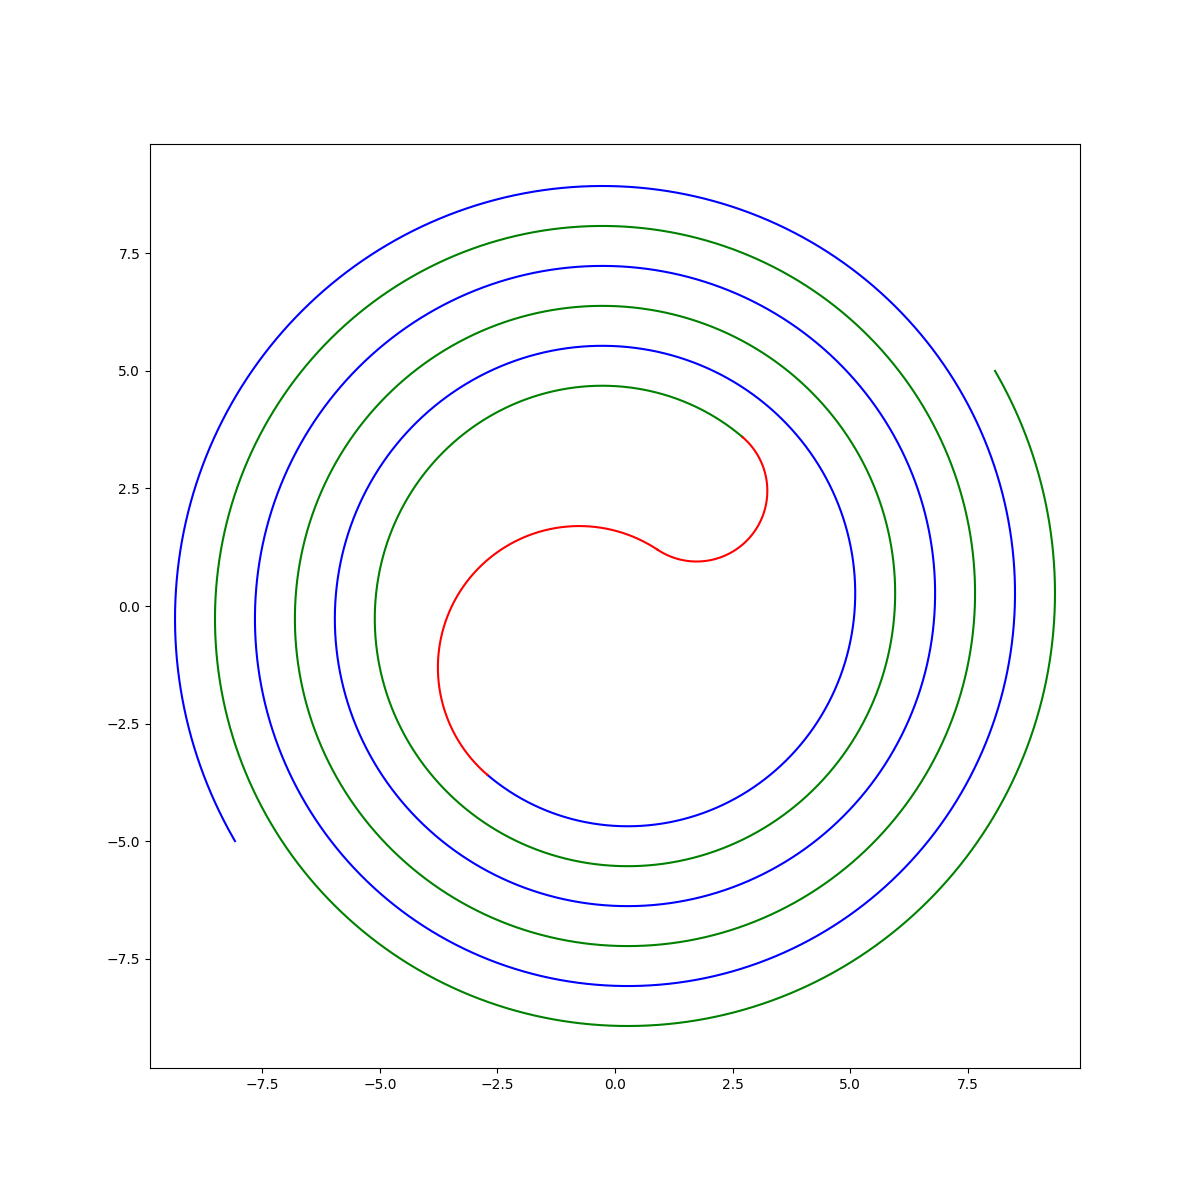
\includegraphics[width=12cm,height=12cm]{figures/q4轨迹.png}	
	\caption{问题四行进轨迹}
\end{figure}
其中蓝色线条为盘入路径，绿色线条为盘出螺线，红色线条为调头圆弧。

通过上方几何模型可以求出盘进圆弧圆心坐标为(-76.00091166555296cm，-130.5726426346256cm)，半径为300.54176677890356cm盘出圆弧圆心坐标为(173.59324901810944cm,244.8401974553665cm)，半径为150.27088338945178cm，从而可获得两个圆弧的方程。

改进问题一的模型：仍采用以上一把手为圆心，以把手间距离为半径的圆与轨迹求交点的方式找出下一点位置。然而，本题中轨迹由四段函数拼接而成，需要确定与哪一个函数进行联立。可以通过以三个函数分段点为圆心分别以龙头两把手距离与龙身两把手距离为半径作圆，可以获得六个分界点，如下图所示：
\begin{figure}[H]
	\label{jmzbx}
	\centering
	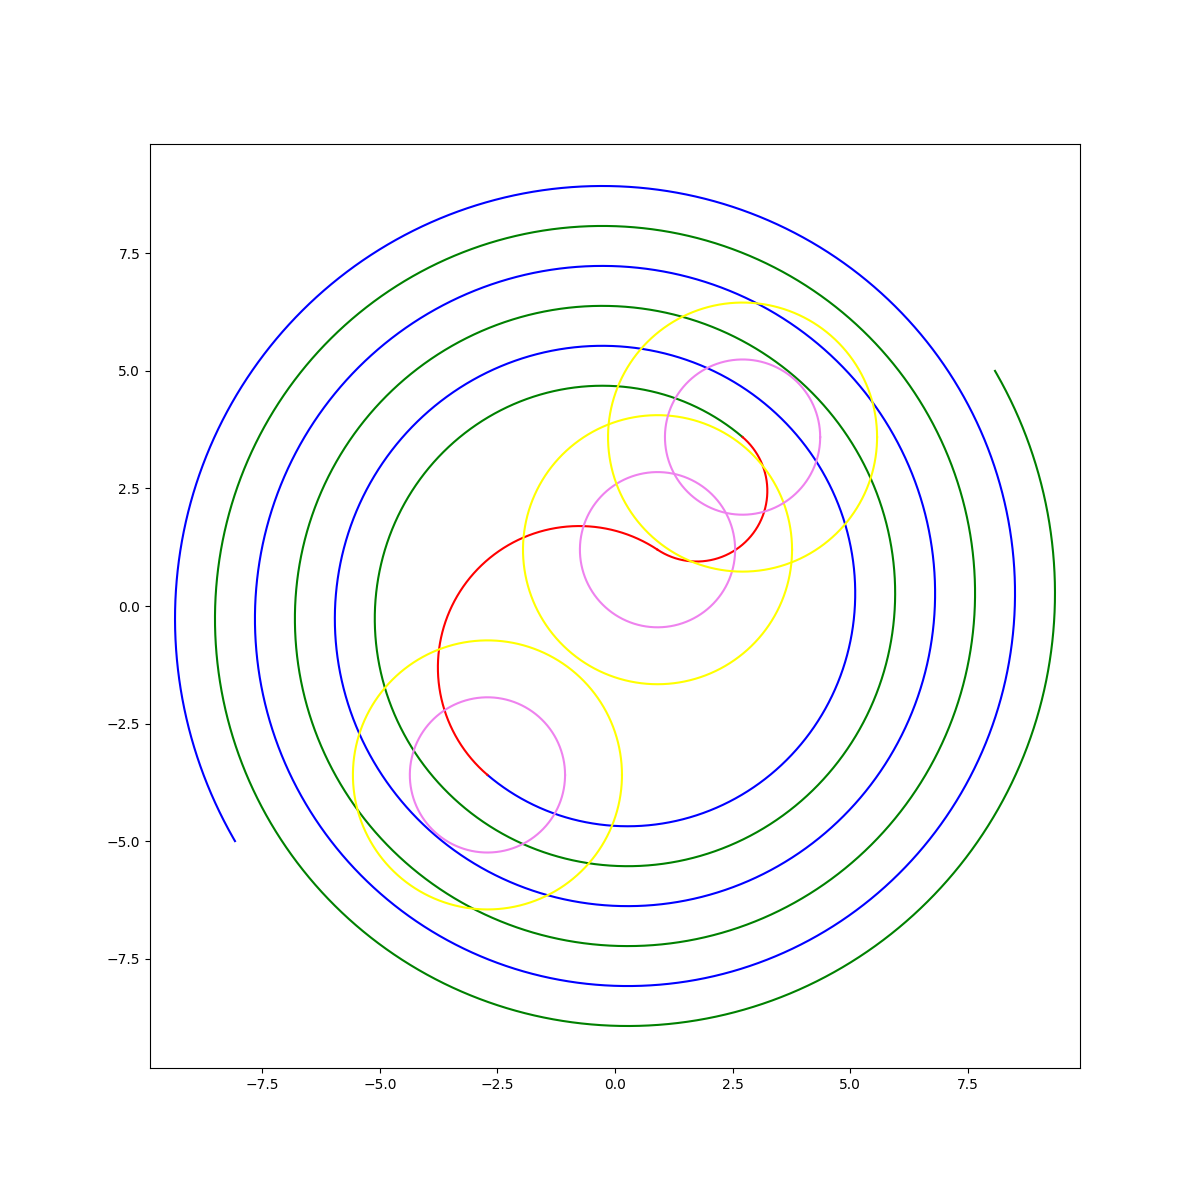
\includegraphics[width=12cm,height=12cm]{figures/q4求分界点.png}	
	\caption{求分界点示意}
\end{figure}
其中粉色圆以龙身把手间距为半径，黄色圆以龙头把手间距为半径。

对于龙头与龙身，均形成了三个有效分界点，将整个轨迹分成四部分，通过判断上一点位于哪一部分之上，从而确定联立与何函数联立，在解中取得一个合理的正解舍去增根，可以求得位置如下表所示：

\begin{table}[H]
	\centering
	\caption{舞龙队位置}
	\begin{tabular}{|c|c|c|c|c|c|}
		\hline
 &-100 s &-50 s &0 s &50 s &100 s \\ \hline
龙头x (m) &7.778034 &6.608301 &-2.711856 &1.332696 &-3.157229 \\ \hline
龙头y (m) &3.717164 &1.898865 &-3.591078 &6.175324 &7.548511 \\ \hline
第1节龙身x (m) &6.209273 &5.366911 &-0.063534 &3.862265 &-0.346890 \\ \hline
第1节龙身y (m) &6.108521 &4.475403 &-4.670888 &4.840828 &8.079166 \\ \hline
第51节龙身x (m) &-10.608038 &-3.629945 &2.459962 &-1.671385 &2.095033 \\ \hline
第51节龙身y (m) &2.831491 &-8.963800 &-7.778145 &-6.076713 &4.033787 \\ \hline
第101节龙身x (m) &-11.922761 &10.125787 &3.008493 &-7.591816 &-7.288774 \\ \hline
第101节龙身y (m) &-4.802378 &-5.972247 &10.108539 &5.175487 &2.063875 \\ \hline
第151节龙身x (m) &-14.351032 &12.974784 &-7.002789 &-4.605165 &9.462513 \\ \hline
第151节龙身y (m) &-1.980993 &-3.810357 &10.337482 &-10.386988 &-3.540357 \\ \hline
第201节龙身x (m) &-11.952942 &10.522509 &-6.872842 &0.336952 &8.524374 \\ \hline
第201节龙身y (m) &10.566998 &-10.807425 &12.382609 &-13.177610 &8.606933 \\ \hline
龙尾（后）x (m) &-1.011059 &0.189809 &-1.933627 &5.859094 &-10.980157 \\ \hline
龙尾（后）y (m) &-16.527573 &15.720588 &-14.713128 &12.612894 &-6.770006 \\ \hline
	\end{tabular}
\end{table}

与问题一类似的，可以求得等距螺线切线的斜率：
$$k=\frac{\mathrm{d} y}{\mathrm{d} x} =\frac{\sin \theta +  \theta \cos \theta }{\cos \theta - \theta \sin \theta }$$
对以($x_{1}$,$y_{1}$)为圆心的圆，其上一点($x_{0}$,$y_{0}$)处的切线斜率为：
$$k=\frac{x_{0}-x_{1}  }{y_{1}-y_{0}  }  $$
进而可求得杆与切线夹角余弦值：
$$\cos \alpha =\frac{\left ( 1,k \right ) \cdot \left ( x_{n+1}-x_{n},y_{n+1}-y_{n} \right ) }{\left | \left ( 1,k \right ) \right | \cdot \left |  \left ( x_{n+1}-x_{n},y_{n+1}-y_{n} \right ) \right | }$$
再带入问题一中公式,考虑延杆速度相同，依次递推求解即可：
\begin{table}[H]
	\centering
	\caption{舞龙队速度}
	\begin{tabular}{|c|c|c|c|c|c|}
		\hline
 &-100 s &-50 s &0 s &50 s &100 s \\ \hline
龙头 (m/s) &1.0 &1.0 &1.0 &1.0 &1.0\\ \hline
第1节龙身  (m/s) &0.999904 &0.999762 &0.998687 &1.000363 &1.000124 \\ \hline
第51节龙身  (m/s) &0.999346 &0.998642 &0.995134 &0.949935 &1.003966 \\ \hline
第101节龙身  (m/s) &0.999091 &0.998248 &0.994448 &0.948482 &1.096263 \\ \hline
第151节龙身  (m/s) &0.998944 &0.998047 &0.994156 &0.948038 &1.095306 \\ \hline
第201节龙身  (m/s) &0.998849 &0.997925 &0.993994 &0.947823 &1.094933 \\ \hline
龙尾（后） (m/s) &0.998817 &0.997885 &0.993944 &0.947760 &1.094833 \\ \hline
	\end{tabular}
\end{table}
\subsection{问题五模型的建立与求解}
观察问题四的速度表格，注意到，在盘出螺线上，对同一节身体，其后把手速度略快于前把手，且速度增量逐渐增大。在掉头区域内，速度发生较大突变，迅速增大。在盘入螺线上，后把手速度略慢于前把手，且速度减少量逐渐减少。t=150s时速度与把手位于龙身的节数的散点图如下：
\begin{figure}[H]
	\label{jmzbx}
	\centering
	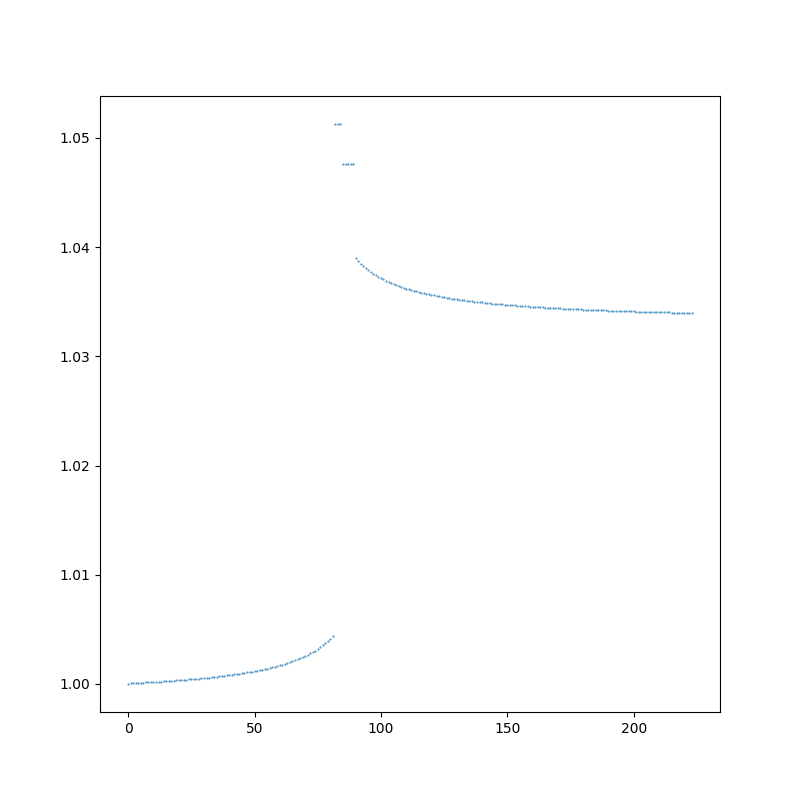
\includegraphics[width=12cm,height=12cm]{figures/把手节数速度关系.png}	
	\caption{t=150s 速度与各把手散点图}
\end{figure}
可以大致确定，整条板凳龙中速度最大的把手恰为正在调头区域上的把手。
此外，固定龙头速度仍为1m/s。以时间为横轴，整条龙上最大把手速度为纵轴画出时间速度：
\begin{figure}[H]
	\label{jmzbx}
	\centering
	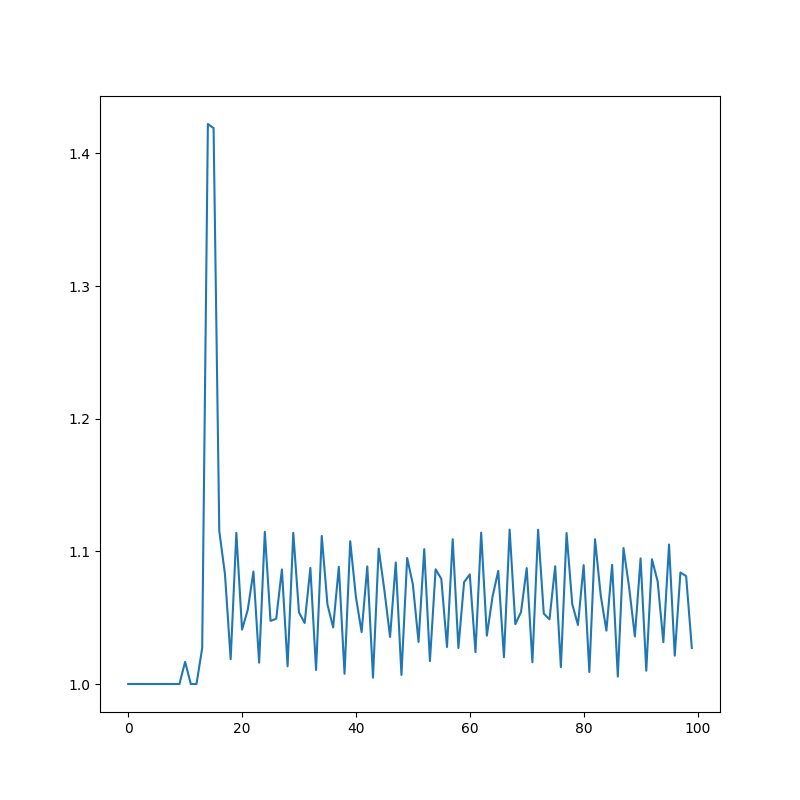
\includegraphics[width=12cm,height=12cm]{figures/时间-vmax.png}	
	\caption{时间与最大速度折线图}
\end{figure}
观察到在t=14s附近速度的极大值最大，即龙身在恰好离开调头区域时，后方仍停留在掉头区域内，且靠近龙头的把手速度最大。据此，我们可以确定达到速度最大值的t位于[13s,15s]内，对此区间进行二分查找，得到t=14.479969063000013s时，龙身把手有最大速度1.60479337899512m/s。

由问题一计算速度的公式，在板凳龙位置固定时，后把手与前把手速度成线性关系，故所有把手均与龙头成线性关系，即
$$\frac{v_{ans}}{1.0m/s}=   \frac{2m/s}{v_{max}}$$
其中$v_{ans}$表示所求速度，$v_{max}$表示上文求得的在固定龙头速度为1m/s的情况下，龙身把手的最大速度

最终求得答案为：$v_{ans}$=1.246266m/s
\section{模型的评价与推广}
\subsection{模型优点}

1.采用递推的方式确定整个舞龙队的位置和速度，对计算复杂度有所优化。

2.在建立模型过程中采用了可视化的方法，能够以较为直观的方式展示整个舞龙队盘入盘出的情况，在模拟进程的同时加上了碰撞检测，减少了不必要的无关量，优化了算法效率。同时采用二分法进行了检验，保证了准确性。

3.各模块区分明显，对于不同的步骤采用不同的代码块，对于相近的步骤则通过改进先前相近的模型实现目的，减少了整个建模的工程量。

4.本模型对于不同的路径可以采用同样的方法计算，具有很强的普适性。

\subsection{模型缺点}

1.计算时忽略了人的反应速度，速度始终同时改变，会对实际结果造成一定的误差。

2.考虑的变量过多，导致计算量较大，程序较为复杂，可以对程序进行优化。

\subsection{模型的改进与推广}

1.在改变速度时，加入人的反应时间，并对速度改变做出一系列延时处理，同时加入延时处理的修正函数，以使结果更加符合实际。

2.可以对模型进行近似，加快求解过程，降低求解复杂度。

\newpage

\bibliography{book}
本文无参考文献

\newpage
%附录
\appendix
\section{支撑文件目录}
\begin{lstlisting}
    result1.xlsx
    result2.xlsx
    result4.xlsx
\end{lstlisting}
\section{问题一位置输出代码}
\begin{lstlisting}[language=python]
    from sympy import *
    import openpyxl

    l_head = 286
    l_body = 165
    a = 27.5 / pi
    r0 = 16 * 55
    v0 = 100


    def ans_site(t):
        ansr = []
        anssita = []
        anssite = []
        r = symbols('r')
        fr = r * sqrt(r * r + a * a) / 2 + a * a * ln(
            (r + sqrt(r * r + a * a)) / (r0 + sqrt(r0 * r0 + a * a))) / 2 - r0 * sqrt(
            r0 * r0 + a * a) / 2 + a * v0 * t
        ansr.append(nsolve(fr, 700))
        anssita.append(ansr[0] / a)
        x0 = ansr[0] * cos(anssita[0])
        y0 = ansr[0] * sin(anssita[0])
        anssite.append(x0.evalf())
        anssite.append(y0.evalf())
        fr = (r * cos(r / a) - x0) *(r * cos(r / a) - x0) + (r * sin(r / a) - y0) *(r * sin(r / a) - y0)- l_head *l_head
        ansr.append(nsolve(fr, ansr[0] + 2))
        anssita.append(ansr[1] / a)
        for i in range(1, 224):
            x0 = ansr[i] * cos(anssita[i])
            y0 = ansr[i] * sin(anssita[i])
            fr = (r * cos(r / a) - x0) *(r * cos(r / a) - x0) + (r * sin(r / a) - y0) *(r * sin(r / a) - y0) - l_body *l_body
            ansr.append(nsolve(fr, ansr[i] + 2))
            anssita.append(ansr[i + 1] / a)
            x = ansr[i] * cos(anssita[i])
            y = ansr[i] * sin(anssita[i])
            anssite.append(x.evalf())
            anssite.append(y.evalf())
        return anssite

    print("ok")
    wb = openpyxl.load_workbook('result1.xlsx')
    sheet = wb['位置']
    for t in range(0, 301):
        ans = ans_site(t)
        for i in range(448):
            tmp = ans[i] / 100
            sheet.cell(i + 2, t + 2).value = str(round(tmp, 6))
    wb.save('result1.xlsx')

\end{lstlisting}

\section{问题一速度输出代码}
\begin{lstlisting}[language=python]
    from sympy import *
    import openpyxl

    l_head = 286
    l_body = 165
    a = 27.5 / pi
    r0 = 16 * 55
    v0 = 100


    def ans_verb(t):
        ansr = []
        anssita = []
        v = []
        v.append(1.000000)
        r = symbols('r')
        fr = r * sqrt(r * r + a * a) / 2 + a * a * ln(
            (r + sqrt(r * r + a * a)) / (r0 + sqrt(r0 * r0 + a * a))) / 2 - r0 * sqrt(
            r0 * r0 + a * a) / 2 + a * v0 * t
        ansr.append(nsolve(fr, 810))
        anssita.append(ansr[0] / a)
        x0 = ansr[0] * cos(anssita[0])
        y0 = ansr[0] * sin(anssita[0])
        fr = (r * cos(r / a) - x0) * (r * cos(r / a) - x0) + (r * sin(r / a) - y0) * (r * sin(r / a) - y0) - l_head * l_head
        ansr.append(nsolve(fr, ansr[0] + 2))
        anssita.append(ansr[1] / a)
        for i in range(1, 223):
            x0 = ansr[i] * cos(anssita[i])
            y0 = ansr[i] * sin(anssita[i])
            fr = (r * cos(r / a) - x0) * (r * cos(r / a) - x0) + (r * sin(r / a) - y0) * (
                    r * sin(r / a) - y0) - l_body * l_body
            ansr.append(nsolve(fr, ansr[i] + 2))
            anssita.append(ansr[i + 1] / a)

        cosbn = (ansr[0] * ansr[0] + l_head * l_head - ansr[1] * ansr[1]) / (2 * ansr[0] * l_head)
        cosan = ansr[0] / sqrt(ansr[0] * ansr[0] + a * a)
        sinan = a / sqrt(ansr[0] * ansr[0] + a * a)
        cosfn1 = (ansr[1] * ansr[1] + l_head * l_head - ansr[0] * ansr[0]) / (2 * ansr[1] * l_head)
        cosan1 = ansr[1] / sqrt(ansr[1] * ansr[1] + a * a)
        sinan1 = a / sqrt(ansr[1] * ansr[1] + a * a)
        nxt = v[0] * (sqrt(1 - cosbn * cosbn) * cosan - cosbn * sinan) / (
                sqrt(1 - cosfn1 * cosfn1) * cosan1 + cosfn1 * sinan1)
        v.append(abs(nxt.evalf()))
        for i in range(1, 223):
            cosbn = (ansr[i] * ansr[i] + l_body * l_body - ansr[i + 1] * ansr[i + 1]) / (2 * ansr[i] * l_body)
            cosan = ansr[i] / sqrt(ansr[i] * ansr[i] + a * a)
            sinan = a / sqrt(ansr[i] * ansr[i] + a * a)
            cosfn1 = (ansr[i + 1] * ansr[i + 1] + l_body * l_body - ansr[i] * ansr[i]) / (2 * ansr[i + 1] * l_body)
            cosan1 = ansr[i + 1] / sqrt(ansr[i + 1] * ansr[i + 1] + a * a)
            sinan1 = a / sqrt(ansr[1 + 1] * ansr[i + 1] + a * a)
            nxt = v[i] * (sqrt(1 - cosbn * cosbn) * cosan - cosbn * sinan) / (
                    sqrt(1 - cosfn1 * cosfn1) * cosan1 + cosfn1 * sinan1)
            v.append(abs(nxt.evalf()))
        return v


    wb = openpyxl.load_workbook('result1.xlsx')
    sheet = wb['速度']
    for t in range(200, 301):
        print(t)
        ans = ans_verb(t)
        for i in range(224):
            sheet.cell(i + 2, t + 2).value = str(round(ans[i], 6))
    wb.save('result1.xlsx')

\end{lstlisting}

\section{问题二可视化代码}
\begin{lstlisting}[language=python]
    import matplotlib.pyplot as plt
    import numpy as np
    import pandas as pd
    import matplotlib.animation as ani

    fig = plt.figure(figsize=(8, 8))
    ax = plt.gca()
    ax.grid()
    ax.set_xlim(-13, 13)
    ax.set_ylim(-13, 13)
    ln1, = ax.plot([], [], '-', lw=2)
    line = []
    line.append(ln1)
    for i in range(1, 101):
        ln, = ax.plot([], [], '-', lw=2)
        line.append(ln)
    df = pd.read_excel('result1.xlsx', sheet_name='位置')


    def update(i):
        column_data = df[str(i) + ' s']
        data_array = column_data.values.tolist()
        x = data_array[::2]
        y = data_array[1::2]
        xi = []
        yi = []
        xpoints = np.array(x)
        ypoints = np.array(y)
        line[0].set_data(xpoints, ypoints)

        xi.clear()
        yi.clear()

        for i in range(1, 100):
            cosx = (x[i + 1] - x[i]) / 1.65
            cosy = (y[i + 1] - y[i]) / 1.65
            x1 = x[i] - 0.275 * cosx
            y1 = y[i] - 0.275 * cosy
            x0 = x1 + 0.15 * cosy
            y0 = y1 - 0.15 * cosx
            xi.append(x0)
            yi.append(y0)
            x0 += 2.20 * cosx
            y0 += 2.20 * cosy
            xi.append(x0)
            yi.append(y0)
            x0 -= 0.3 * cosy
            y0 += 0.3 * cosx
            xi.append(x0)
            yi.append(y0)
            x0 -= 2.20 * cosx
            y0 -= 2.20 * cosy
            xi.append(x0)
            yi.append(y0)
            x0 += 0.3 * cosy
            y0 -= 0.3 * cosx
            xi.append(x0)
            yi.append(y0)
            xpoints = np.array(xi)
            ypoints = np.array(yi)
            line[i].set_data(xpoints, ypoints)
            xi.clear()
            yi.clear()
        cosx0=(x[1]-x[0])/2.86
        cosy0=(y[1]-y[0])/2.86
        x1=x[0]-0.275*cosx0
        y1=y[0]-0.275*cosy0
        x0=x1+0.15*cosy0
        y0=y1-0.15*cosx0
        xi.append(x0)
        yi.append(y0)
        x0+=3.41*cosx0
        y0+=3.41*cosy0
        xi.append(x0)
        yi.append(y0)
        x0-=0.3*cosy0
        y0+=0.3*cosx0
        xi.append(x0)
        yi.append(y0)
        x0-=3.41*cosx0
        y0-=3.41*cosy0
        xi.append(x0)
        yi.append(y0)
        x0+=0.3*cosy0
        y0-=0.3*cosx0
        xi.append(x0)
        yi.append(y0)
        xpoints = np.array(xi)
        ypoints = np.array(yi)
        line[i].set_data(xpoints, ypoints)
        xi.clear()
        yi.clear()
        return line


    animation = ani.FuncAnimation(fig, update, range(0, 301), interval=100)

    plt.show()

\end{lstlisting}

\section{问题二二分查找代码}
\begin{lstlisting}[language=python]
    from sympy import *
    eps = 1e-12
    l_head = 286
    l_body = 165
    a = 27.5 / pi
    r0 = 16 * 55
    v0 = 100


    def ans_site(t):
        ansr = []
        anssita = []
        anssite = []
        r = symbols('r')
        fr = r * sqrt(r * r + a * a) / 2 + a * a * ln(
            (r + sqrt(r * r + a * a)) / (r0 + sqrt(r0 * r0 + a * a))) / 2 - r0 * sqrt(
            r0 * r0 + a * a) / 2 + a * v0 * t
        ansr.append(nsolve(fr, 700))
        anssita.append(ansr[0] / a)
        x0 = ansr[0] * cos(anssita[0])
        y0 = ansr[0] * sin(anssita[0])
        anssite.append(x0.evalf())
        anssite.append(y0.evalf())
        fr = (r * cos(r / a) - x0) *(r * cos(r / a) - x0) + (r * sin(r / a) - y0) *(r * sin(r / a) - y0)- l_head *l_head
        ansr.append(nsolve(fr, ansr[0] + 2))
        anssita.append(ansr[1] / a)
        for i in range(1, 224):
            x0 = ansr[i] * cos(anssita[i])
            y0 = ansr[i] * sin(anssita[i])
            fr = (r * cos(r / a) - x0) *(r * cos(r / a) - x0) + (r * sin(r / a) - y0) *(r * sin(r / a) - y0) - l_body *l_body
            ansr.append(nsolve(fr, ansr[i] + 2))
            anssita.append(ansr[i + 1] / a)
            x = ansr[i] * cos(anssita[i])
            y = ansr[i] * sin(anssita[i])
            anssite.append(x.evalf())
            anssite.append(y.evalf())
        return anssite
    def bin_search(left,right):
        mid = (left+right)/2
        ans=ans_site(mid)
        cosx0=(ans[2]-ans[0])/2.86
        cosy0=(ans[3]-ans[1])/2.86
        x1=ans[0]-0.275*cosx0
        y1=ans[1]-0.275*cosy0
        x0=x1+0.15*cosy0
        y0=y1-0.15*cosx0
        dis = distance(x0,y0,ans[16],ans[17],ans[18],ans[19])
        print(dis)
        if -eps<dis-15<eps:
            return mid
        elif dis-15<0:
            return bin_search(left,mid)
        else:
            return bin_search(mid,right)
    def distance(x0,y0,x1,y1,x2,y2):
        dis = abs(x0*(y2-y1)+y0*(x1-x2)+(x2*y1-x1*y2))/sqrt((y1-y2)*(y1-y2)+(x1-x2)*(x1-x2))
        return dis

    print(bin_search(412,414))
\end{lstlisting}

\section{问题二位置输出代码}
\begin{lstlisting}[language=python]
    from sympy import *
    import openpyxl

    l_head = 286
    l_body = 165
    a = 27.5 / pi
    r0 = 16 * 55
    v0 = 100


    def ans_site(t):
        ansr = []
        anssita = []
        anssite = []
        r = symbols('r')
        fr = r * sqrt(r * r + a * a) / 2 + a * a * ln(
            (r + sqrt(r * r + a * a)) / (r0 + sqrt(r0 * r0 + a * a))) / 2 - r0 * sqrt(
            r0 * r0 + a * a) / 2 + a * v0 * t
        ansr.append(nsolve(fr, 700))
        anssita.append(ansr[0] / a)
        x0 = ansr[0] * cos(anssita[0])
        y0 = ansr[0] * sin(anssita[0])
        anssite.append(x0.evalf())
        anssite.append(y0.evalf())
        fr = (r * cos(r / a) - x0) * (r * cos(r / a) - x0) + (r * sin(r / a) - y0) * (r * sin(r / a) - y0) - l_head * l_head
        ansr.append(nsolve(fr, ansr[0] + 2))
        anssita.append(ansr[1] / a)
        for i in range(1, 224):
            x0 = ansr[i] * cos(anssita[i])
            y0 = ansr[i] * sin(anssita[i])
            fr = (r * cos(r / a) - x0) * (r * cos(r / a) - x0) + (r * sin(r / a) - y0) * (
                    r * sin(r / a) - y0) - l_body * l_body
            ansr.append(nsolve(fr, ansr[i] + 2))
            anssita.append(ansr[i + 1] / a)
            x = ansr[i] * cos(anssita[i])
            y = ansr[i] * sin(anssita[i])
            anssite.append(x.evalf())
            anssite.append(y.evalf())
        return anssite


    wb = openpyxl.load_workbook('result2.xlsx')
    sheet = wb['Sheet1']
    ans = ans_site(412.473837)
    for i in range(224):
        tmp1 = ans[2 * i] / 100
        tmp2 = ans[2 * i + 1] / 100
        sheet.cell(i + 2, 2).value = str(round(tmp1, 6))
        sheet.cell(i + 2, 3).value = str(round(tmp2, 6))
    wb.save('result2.xlsx')

\end{lstlisting}

\section{问题二速度输出代码}
\begin{lstlisting}[language=python]
    from sympy import *
    import openpyxl

    l_head = 286
    l_body = 165
    a = 27.5 / pi
    r0 = 16 * 55
    v0 = 100


    def ans_verb(t):
        ansr = []
        anssita = []
        v = []
        v.append(1.000000)
        r = symbols('r')
        fr = r * sqrt(r * r + a * a) / 2 + a * a * ln(
            (r + sqrt(r * r + a * a)) / (r0 + sqrt(r0 * r0 + a * a))) / 2 - r0 * sqrt(
            r0 * r0 + a * a) / 2 + a * v0 * t
        ansr.append(nsolve(fr, 810))
        anssita.append(ansr[0] / a)
        x0 = ansr[0] * cos(anssita[0])
        y0 = ansr[0] * sin(anssita[0])
        fr = (r * cos(r / a) - x0) * (r * cos(r / a) - x0) + (r * sin(r / a) - y0) * (r * sin(r / a) - y0) - l_head * l_head
        ansr.append(nsolve(fr, ansr[0] + 2))
        anssita.append(ansr[1] / a)
        for i in range(1, 223):
            x0 = ansr[i] * cos(anssita[i])
            y0 = ansr[i] * sin(anssita[i])
            fr = (r * cos(r / a) - x0) * (r * cos(r / a) - x0) + (r * sin(r / a) - y0) * (
                    r * sin(r / a) - y0) - l_body * l_body
            ansr.append(nsolve(fr, ansr[i] + 2))
            anssita.append(ansr[i + 1] / a)

        cosbn = (ansr[0] * ansr[0] + l_head * l_head - ansr[1] * ansr[1]) / (2 * ansr[0] * l_head)
        cosan = ansr[0] / sqrt(ansr[0] * ansr[0] + a * a)
        sinan = a / sqrt(ansr[0] * ansr[0] + a * a)
        cosfn1 = (ansr[1] * ansr[1] + l_head * l_head - ansr[0] * ansr[0]) / (2 * ansr[1] * l_head)
        cosan1 = ansr[1] / sqrt(ansr[1] * ansr[1] + a * a)
        sinan1 = a / sqrt(ansr[1] * ansr[1] + a * a)
        nxt = v[0] * (sqrt(1 - cosbn * cosbn) * cosan - cosbn * sinan) / (
                sqrt(1 - cosfn1 * cosfn1) * cosan1 + cosfn1 * sinan1)
        v.append(abs(nxt.evalf()))
        for i in range(1, 223):
            cosbn = (ansr[i] * ansr[i] + l_body * l_body - ansr[i + 1] * ansr[i + 1]) / (2 * ansr[i] * l_body)
            cosan = ansr[i] / sqrt(ansr[i] * ansr[i] + a * a)
            sinan = a / sqrt(ansr[i] * ansr[i] + a * a)
            cosfn1 = (ansr[i + 1] * ansr[i + 1] + l_body * l_body - ansr[i] * ansr[i]) / (2 * ansr[i + 1] * l_body)
            cosan1 = ansr[i + 1] / sqrt(ansr[i + 1] * ansr[i + 1] + a * a)
            sinan1 = a / sqrt(ansr[1 + 1] * ansr[i + 1] + a * a)
            nxt = v[i] * (sqrt(1 - cosbn * cosbn) * cosan - cosbn * sinan) / (
                    sqrt(1 - cosfn1 * cosfn1) * cosan1 + cosfn1 * sinan1)
            v.append(abs(nxt.evalf()))
        return v


    wb = openpyxl.load_workbook('result2.xlsx')
    sheet = wb['Sheet1']
    ans = ans_verb(412.473837)
    for i in range(224):
        sheet.cell(i + 2, 4).value = str(round(ans[i], 6))
    wb.save('result2.xlsx')


\end{lstlisting}

\section{问题三可视化代码}
\begin{lstlisting}[language=python]
    import matplotlib.pyplot as plt
    import numpy as np
    import pandas as pd
    import matplotlib.animation as ani

    fig = plt.figure(figsize=(8, 8))
    ax = plt.gca()
    ax.grid()
    ax.set_xlim(-13, 13)
    ax.set_ylim(-13, 13)
    ln1, = ax.plot([], [], '-', lw=2)
    line = []
    line.append(ln1)
    time_template = 'a = %.1f cm/rad'
    time_text = ax.text(0.05, 0.9, '', transform=ax.transAxes)
    for i in range(1, 101):
        ln, = ax.plot([], [], '-', lw=2)
        line.append(ln)
    df = pd.read_excel('plot.xlsx', sheet_name='位置')


    def update(j):
        column_data = df[str(j) + ' s']
        data_array = column_data.values.tolist()
        x = data_array[::2]
        y = data_array[1::2]
        xi = []
        yi = []
        xpoints = np.array(x)
        ypoints = np.array(y)
        line[0].set_data(xpoints, ypoints)

        xi.clear()
        yi.clear()

        for i in range(1, 100):
            cosx = (x[i + 1] - x[i]) / 1.65
            cosy = (y[i + 1] - y[i]) / 1.65
            x1 = x[i] - 0.275 * cosx
            y1 = y[i] - 0.275 * cosy
            x0 = x1 + 0.15 * cosy
            y0 = y1 - 0.15 * cosx
            xi.append(x0)
            yi.append(y0)
            x0 += 2.20 * cosx
            y0 += 2.20 * cosy
            xi.append(x0)
            yi.append(y0)
            x0 -= 0.3 * cosy
            y0 += 0.3 * cosx
            xi.append(x0)
            yi.append(y0)
            x0 -= 2.20 * cosx
            y0 -= 2.20 * cosy
            xi.append(x0)
            yi.append(y0)
            x0 += 0.3 * cosy
            y0 -= 0.3 * cosx
            xi.append(x0)
            yi.append(y0)
            xpoints = np.array(xi)
            ypoints = np.array(yi)
            line[i].set_data(xpoints, ypoints)
            xi.clear()
            yi.clear()
        cosx0=(x[1]-x[0])/2.86
        cosy0=(y[1]-y[0])/2.86
        x1=x[0]-0.275*cosx0
        y1=y[0]-0.275*cosy0
        x0=x1+0.15*cosy0
        y0=y1-0.15*cosx0
        xi.append(x0)
        yi.append(y0)
        x0+=3.41*cosx0
        y0+=3.41*cosy0
        xi.append(x0)
        yi.append(y0)
        x0-=0.3*cosy0
        y0+=0.3*cosx0
        xi.append(x0)
        yi.append(y0)
        x0-=3.41*cosx0
        y0-=3.41*cosy0
        xi.append(x0)
        yi.append(y0)
        x0+=0.3*cosy0
        y0-=0.3*cosx0
        xi.append(x0)
        yi.append(y0)
        xpoints = np.array(xi)
        ypoints = np.array(yi)
        line[i].set_data(xpoints, ypoints)
        xi.clear()
        yi.clear()
        time_text.set_text(time_template %(2+j*0.1))
        return line, time_text

    animation = ani.FuncAnimation(fig, update, range(50,65), interval=1000)

    plt.show()

\end{lstlisting}

\section{问题三碰撞检测代码}
\begin{lstlisting}[language=python]
    from sympy import *
    import numpy as np
    import matplotlib.pyplot as plt

    eps = 1e-12
    l_head = 286
    l_body = 165


    def ans_site(a, r0):
        ansr = []
        anssita = []
        anssite = []
        r = symbols('r')
        fr = r * sqrt(r * r + a * a) / 2 + a * a * ln(
            (r + sqrt(r * r + a * a)) / (r0 + sqrt(r0 * r0 + a * a))) / 2 - r0 * sqrt(
            r0 * r0 + a * a) / 2
        ansr.append(nsolve(fr, 700))
        anssita.append(ansr[0] / a)
        x0 = ansr[0] * cos(anssita[0])
        y0 = ansr[0] * sin(anssita[0])
        anssite.append([x0.evalf(), y0.evalf()])
        fr = (r * cos(r / a) - x0) * (r * cos(r / a) - x0) + (r * sin(r / a) - y0) * (r * sin(r / a) - y0) - l_head * l_head
        ansr.append(nsolve(fr, ansr[0] + 2))
        anssita.append(ansr[1] / a)
        for i in range(1, 224):
            x0 = ansr[i] * cos(anssita[i])
            y0 = ansr[i] * sin(anssita[i])
            fr = (r * cos(r / a) - x0) * (r * cos(r / a) - x0) + (r * sin(r / a) - y0) * (
                    r * sin(r / a) - y0) - l_body * l_body
            ansr.append(nsolve(fr, ansr[i] + 2))
            anssita.append(ansr[i + 1] / a)
            x = ansr[i] * cos(anssita[i])
            y = ansr[i] * sin(anssita[i])
            anssite.append([x.evalf(), y.evalf()])
        return anssite


    def distance(x0, y0, x1, y1, x2, y2):
        dis = abs(x0 * (y2 - y1) + y0 * (x1 - x2) + (x2 * y1 - x1 * y2)) / sqrt(
            (y1 - y2) * (y1 - y2) + (x1 - x2) * (x1 - x2))
        return dis


    r = np.arange(462.44, 462.46, 0.002)
    a = np.arange(7.158871, 7.1588715, 0.00000005)
    for i in a:
        print("a="+str(i),end=':')
        for j in r:
            ans = ans_site(i, j)
            cosx0 = (ans[1][0] - ans[0][0]) / 2.86
            cosy0 = (ans[1][1] - ans[0][1]) / 2.86
            x1 = ans[0][0] - 0.275 * cosx0
            y1 = ans[0][1] - 0.275 * cosy0
            x0 = x1 + 0.15 * cosy0
            y0 = y1 - 0.15 * cosx0
            if distance(x0, y0, ans[17][0], ans[17][1], ans[18][0], ans[18][1]) > 15:
                print(0,end=' ')
            else:
                print(1,end=' ')
        print()

\end{lstlisting}

\section{问题四位置输出代码}
\begin{lstlisting}[language=python]
    from sympy import *
    import openpyxl
    import numpy as np
    import math
    l_head = 286
    l_body = 165
    r0 = 450
    a = 85 / np.pi
    v0 = 100
    theta0 = r0 / a
    a0 = -np.arctan((np.sin(r0 / a) + (r0 / a) * np.cos(r0 / a)) / (np.cos(r0 / a) - (r0 / a) * np.sin(r0 / a)))
    b0 = np.arctan(np.tan(r0 / a))
    r1 = 2 * math.sqrt(r0 * r0 + a * a) / 3
    r2 = math.sqrt(r0 * r0 + a * a) / 3
    x1 = r0 * np.cos(theta0) + r1 * np.sin(a0)
    y1 = r0 * np.sin(theta0) + r1 * np.cos(a0)  # 大圆心
    x2 = -r0 * np.cos(theta0) - r2 * np.sin(a0)
    y2 = -r0 * np.sin(theta0) - r2 * np.cos(a0)  # 小圆心
    xc = -r0 * np.cos(theta0) / 3
    yc = -r0 * np.sin(theta0) / 3  # 两圆交点
    eps = 0.1
    def archway_length(xc, yc, x1, y1, x2, y2, r):
        (x1 - xc) * (x2 - xc) + (y1 - yc) * (y2 - yc)
        theta = acos(((x1 - xc) * (x2 - xc) + (y1 - yc) * (y2 - yc)) / r / r)
        return r * theta
    len1 = archway_length(x1, y1, r0 * np.cos(theta0), r0 * np.sin(theta0), xc, yc, r1)
    len2 = archway_length(x2, y2, -r0 * np.cos(theta0), -r0 * np.sin(theta0), xc, yc, r2)

    def location(t):
        if t < 0:
            s = v0 * t
            r = symbols('r')
            fr = r * sqrt(r * r + a * a) / 2 + a * a * ln(
                (r + sqrt(r * r + a * a)) / (r0 + sqrt(r0 * r0 + a * a))) / 2 - r0 * sqrt(
                r0 * r0 + a * a) / 2 + a * s
            r = nsolve(fr, r0 + 2)
            x = r * cos(r / a)
            y = r * sin(r / a)
            return [x, y]
        elif v0 * t <= len1:
            if r0 * np.sin(theta0) > y1:
                a1 = np.arccos((r0 * np.cos(theta0) - x1) / r1)
            else:
                a1 = 2 * np.pi - np.arccos((r0 * np.cos(theta0) - x1) / r1)
            theta = a1 - v0 * t / r1
            x = x1 + r1 * cos(theta)
            y = y1 + r1 * sin(theta)
            return [x, y]
        elif v0 * t <= len1 + len2:
            if -r0 * np.sin(theta0) / 3 > y2:
                a1 = np.arccos((-r0 * np.cos(theta0) / 3 - x2) / r2)
            else:
                a1 = 2 * np.pi - np.arccos((-r0 * np.cos(theta0) / 3 - x2) / r2)
            theta = a1 + (v0 * t -len1) / r2
            x = x2 + r2 * cos(theta)
            y = y2 + r2 * sin(theta)
            return [x, y]
        else:
            s = v0 * t - len1 - len2
            r = symbols('r')
            fr = r * sqrt(r * r + a * a) / 2 + a * a * ln(
                (r + sqrt(r * r + a * a)) / (r0 + sqrt(r0 * r0 + a * a))) / 2 - r0 * sqrt(
                r0 * r0 + a * a) / 2 - a * s
            r = nsolve(fr, r0 + 2)
            x = r * cos(r / a)
            y = r * sin(r / a)
            return [-x, -y]

    def ans_site(t):
        ansr = []
        anssita = []
        anssite = []
        if(t<=0):
            s = v0 * t
            r = symbols('r')
            fr = r * sqrt(r * r + a * a) / 2 + a * a * ln(
                (r + sqrt(r * r + a * a)) / (r0 + sqrt(r0 * r0 + a * a))) / 2 - r0 * sqrt(
                r0 * r0 + a * a) / 2 + a * s
            r = nsolve(fr, r0 + 2)
            ansr.append(r)
            anssita.append(ansr[0]/a)
            anssite.append(ansr[0]*cos(anssita[0]))
            anssite.append(ansr[0] * sin(anssita[0]))
        elif(t<=(len1+len2)/v0):
            site=location(t)
            x0 = site[0]
            y0 = site[1]
            anssite.append(x0)
            anssite.append(y0)
            ansr.append(sqrt(x0*x0+y0*y0))
            theta = atan(y0/x0)
            if (x0 <= 0):
                theta += pi
            anssita.append(theta)
        else:
            s = v0 * t - len1 - len2
            r = symbols('r')
            fr = r * sqrt(r * r + a * a) / 2 + a * a * ln(
                (r + sqrt(r * r + a * a)) / (r0 + sqrt(r0 * r0 + a * a))) / 2 - r0 * sqrt(
                r0 * r0 + a * a) / 2 - a * s
            r = nsolve(fr, r0 + 2)
            ansr.append(r)
            anssita.append(ansr[0]/a+pi)
            anssite.append(ansr[0]*cos(anssita[0]))
            anssite.append(ansr[0] * sin(anssita[0]))
        x0=anssite[0]
        y0=anssite[1]
        print(ansr[0]-a*anssita[0])
        if((-eps<ansr[0]-a*anssita[0]<eps and ansr[0]>=450) or (ansr[0]<=450 and y0<=-92.2623184486086)):

            r = symbols('r')
            fr = (r * cos(r / a) - x0) *(r * cos(r / a) - x0) + (r * sin(r / a) - y0) *(r * sin(r / a) - y0)- l_head *l_head
            ansr.append(nsolve(fr, max(ansr[0]+1,450)))
            anssita.append(ansr[1]/a)
            ansx = ansr[1] * cos(anssita[1])
            ansy = ansr[1] * sin(anssita[1])
            anssite.append(ansx.evalf())
            anssite.append(ansy.evalf())
            print([ansx.evalf(),ansy.evalf()])
        elif(ansr[0]<=450 and y0<=297.686140859912):
            k=(x1-x0)/(y0-y1)
            b=(x0*x0-x1*x1+y0*y0-y1*y1+r1*r1-l_head*l_head)/(2*(y0-y1))
            tmpa = 1+k*k
            tmpb =2*k*(b-y0) - 2*x0
            tmpc = x0*x0+(b-y0)*(b-y0)-l_head*l_head
            ansx1 = (-tmpb+sqrt(tmpb*tmpb-4*tmpa*tmpc))/(2*tmpa)
            ansy1 = k*ansx1+b
            ansx2 = (-tmpb-sqrt(tmpb*tmpb-4*tmpa*tmpc))/(2*tmpa)
            ansy2 = k*ansx2+b
            theta1 = atan(ansy1/ansx1)
            if(ansx1<=0):
                theta1 += pi
            theta2 = atan(ansy2/ansx2)
            if(ansx2 <= 0):
                theta2 += pi
            if(theta1>anssita[0] and ansy1 > ansx1*tan(r0/a)):
                ansx = ansx1
                ansy = ansy1
            else:
                ansx = ansx2
                ansy = ansy2
            ansx = ansx.evalf()
            anssite.append(ansx)
            ansy = ansy.evalf()
            anssite.append(ansy)
            ansr.append(sqrt(ansx*ansx+ansy*ansy))
            theta = atan(ansy/ansx)
            if(ansx<=0):
                theta += pi
            anssita.append(theta)
        elif(ansr[0]<=467.131999862687):
            k=(x2-x0)/(y0-y2)
            b=(x0*x0-x2*x2+y0*y0-y2*y2+r2*r2-l_head*l_head)/(2*(y0-y2))
            tmpa = 1+k*k
            tmpb =2*k*(b-y0) - 2*x0
            tmpc = x0*x0+(b-y0)*(b-y0)-l_head*l_head
            ansx1 = (-tmpb+sqrt(tmpb*tmpb-4*tmpa*tmpc))/(2*tmpa)
            ansy1 = k*ansx1+b
            ansx2 = (-tmpb-sqrt(tmpb*tmpb-4*tmpa*tmpc))/(2*tmpa)
            ansy2 = k*ansx2+b
            ansr1 = sqrt(ansx1*ansx1+ansy1*ansy1)
            ansr2 = sqrt(ansx2*ansx2+ansy2*ansy2)
            if(ansr1<ansr[0] and ansy1 < ansx1*tan(r0/a)):
                ansx = ansx1
                ansy = ansy1
            else:
                ansx = ansx2
                ansy = ansy2
            
            ansx=ansx.evalf()
            anssite.append(ansx)
            ansy = ansy.evalf()
            anssite.append(ansy)
            ansr.append(sqrt(ansx*ansx+ansy*ansy))
            theta = atan(ansy/ansx)
            if(ansx<=0):
                theta += pi
            anssita.append(theta)
        else:
            r = symbols('r')
            fr = (r * cos(r /a+pi) - x0) *(r * cos(r /a+pi) - x0) + (r * sin(r / a+pi) - y0) *(r * sin(r / a+pi) - y0)- l_head *l_head
            ansr.append(nsolve(fr, ansr[0] - 2))
            anssita.append(ansr[1]/a+pi)
            ansx = ansr[1] * cos(anssita[1])
            ansy = ansr[1] * sin(anssita[1])
            anssite.append(ansx.evalf())
            anssite.append(ansy.evalf())
        for i in range(1, 224):
            x0 = ansr[i] * cos(anssita[i])
            y0 = ansr[i] * sin(anssita[i])
            if((-eps<ansr[i]-a*anssita[i]<eps and ansr[i]>=450)or (ansr[i]<=450 and y0<=-221.624651082794)):
                r = symbols('r')
                fr = (r * cos(r / a) - x0) *(r * cos(r / a) - x0) + (r * sin(r / a) - y0) *(r * sin(r / a) - y0)- l_body *l_body
                ansr.append(nsolve(fr, max(ansr[i]+2,450)))
                anssita.append(ansr[i+1]/a)
                ansx = ansr[i+1] * cos(anssita[i+1])
                ansy = ansr[i+1] * sin(anssita[i+1])
                anssite.append(ansx.evalf())
                anssite.append(ansy.evalf())
            elif(y0<=250 and x0<=255.392637737839 and ansr[i]<=450):
                k=(x1-x0)/(y0-y1)
                b=(x0*x0-x1*x1+y0*y0-y1*y1+r1*r1-l_body*l_body)/(2*(y0-y1))
                tmpa = 1+k*k
                tmpb =2*k*(b-y0) - 2*x0
                tmpc = x0*x0+(b-y0)*(b-y0)-l_body*l_body
                ansx1 = (-tmpb+sqrt(tmpb*tmpb-4*tmpa*tmpc))/(2*tmpa)
                ansy1 = k*ansx1+b
                ansx2 = (-tmpb-sqrt(tmpb*tmpb-4*tmpa*tmpc))/(2*tmpa)
                ansy2 = k*ansx2+b
                theta1 = atan(ansy1/ansx1)
                if(ansx1<=0):
                    theta1 += pi
                theta2 = atan(ansy2/ansx2)
                if(ansx2 <= 0):
                    theta2 += pi
                if(theta1>anssita[i] and ansy1 > ansx1*tan(r0/a)):
                    ansx = ansx1
                    ansy = ansy1
                else:
                    ansx = ansx2
                    ansy = ansy2
                
                ansx=ansx.evalf()
                anssite.append(ansx)
                ansy = ansy.evalf()
                anssite.append(ansy)
                ansr.append(sqrt(ansx*ansx+ansy*ansy))
                theta = atan(ansy/ansx)
                if(ansx<=0):
                    theta += pi
                anssita.append(theta)
            elif(ansr[i]<=459.850636532029):
                k=(x2-x0)/(y0-y2)
                b=(x0*x0-x2*x2+y0*y0-y2*y2+r2*r2-l_body*l_body)/(2*(y0-y2))
                tmpa = 1+k*k
                tmpb =2*k*(b-y0) - 2*x0
                tmpc = x0*x0+(b-y0)*(b-y0)-l_body*l_body
                ansx1 = (-tmpb+sqrt(tmpb*tmpb-4*tmpa*tmpc))/(2*tmpa)
                ansy1 = k*ansx1+b
                ansx2 = (-tmpb-sqrt(tmpb*tmpb-4*tmpa*tmpc))/(2*tmpa)
                ansy2 = k*ansx2+b
                ansr1 = sqrt(ansx1*ansx1+ansy1*ansy1)
                ansr2 = sqrt(ansx2*ansx2+ansy2*ansy2)
                if(ansr1<ansr[i] and ansy1 < ansx1*tan(r0/a)):
                    ansx = ansx1
                    ansy = ansy1
                else:
                    ansx = ansx2
                    ansy = ansy2
                
                ansx=ansx.evalf()
                anssite.append(ansx)
                ansy = ansy.evalf()
                anssite.append(ansy)
                ansr.append(sqrt(ansx*ansx+ansy*ansy))
                theta = atan(ansy/ansx)
                if(ansx<=0):
                    theta += pi
                anssita.append(theta)
            else:
                r = symbols('r')
                fr = (r * cos(r /a+pi) - x0) *(r * cos(r /a+pi) - x0) + (r * sin(r / a+pi) - y0) *(r * sin(r / a+pi) - y0)- l_body *l_body
                ansr.append(nsolve(fr, ansr[i] - 2))
                anssita.append(ansr[i+1]/a+pi)
                ansx = ansr[i+1] * cos(anssita[i+1])
                ansy = ansr[i+1] * sin(anssita[i+1])
                anssite.append(ansx.evalf())
                anssite.append(ansy.evalf())
        return anssite
    wb = openpyxl.load_workbook('result4.xlsx')
    sheet = wb['位置']
    t=10
    while(t<=100):
        ans = ans_site(t)
        for i in range(448):
            tmp = ans[i] / 100
            sheet.cell(i + 2, int(t+100+2)).value = str(round(tmp, 6))
        t+=1
    wb.save('result4.xlsx')

\end{lstlisting}

\section{问题四速度输出代码}
\begin{lstlisting}[language=python]
    import numpy as np
    import math
    from sympy import *
    import openpyxl
    import pandas as pd

    eps = 0.1
    l_head = 286
    l_body = 165
    r0 = 450
    a = 85 / np.pi
    v0 = 100
    theta0 = r0 / a
    a0 = -np.arctan((np.sin(r0 / a) + (r0 / a) * np.cos(r0 / a)) / (np.cos(r0 / a) - (r0 / a) * np.sin(r0 / a)))
    b0 = np.arctan(np.tan(r0 / a))
    r1 = 2 * math.sqrt(r0 * r0 + a * a) / 3
    r2 = math.sqrt(r0 * r0 + a * a) / 3
    x1 = r0 * np.cos(theta0) + r1 * np.sin(a0)
    y1 = r0 * np.sin(theta0) + r1 * np.cos(a0)  # 大圆心
    x2 = -r0 * np.cos(theta0) - r2 * np.sin(a0)
    y2 = -r0 * np.sin(theta0) - r2 * np.cos(a0)  # 小圆心
    xc = -r0 * np.cos(theta0) / 3
    yc = -r0 * np.sin(theta0) / 3  # 两圆交点
    v = []
    v.append(1)
    site = []


    def ans_site(t):
        ansr = []
        anssita = []
        anssite = []
        if (t <= 0):
            s = v0 * t
            r = symbols('r')
            fr = r * sqrt(r * r + a * a) / 2 + a * a * ln(
                (r + sqrt(r * r + a * a)) / (r0 + sqrt(r0 * r0 + a * a))) / 2 - r0 * sqrt(
                r0 * r0 + a * a) / 2 + a * s
            r = nsolve(fr, r0 + 2)
            ansr.append(r)
            anssita.append(ansr[0] / a)
            anssite.append(ansr[0] * cos(anssita[0]))
            anssite.append(ansr[0] * sin(anssita[0]))
        elif (t <= (len1 + len2) / v0):
            site = location(t)
            x0 = site[0]
            y0 = site[1]
            anssite.append(x0)
            anssite.append(y0)
            ansr.append(sqrt(x0 * x0 + y0 * y0))
            theta = atan(y0 / x0)
            if (x0 <= 0):
                theta += pi
            anssita.append(theta)
        else:
            s = v0 * t - len1 - len2
            r = symbols('r')
            fr = r * sqrt(r * r + a * a) / 2 + a * a * ln(
                (r + sqrt(r * r + a * a)) / (r0 + sqrt(r0 * r0 + a * a))) / 2 - r0 * sqrt(
                r0 * r0 + a * a) / 2 - a * s
            r = nsolve(fr, r0 + 2)
            ansr.append(r)
            anssita.append(ansr[0] / a + pi)
            anssite.append(ansr[0] * cos(anssita[0]))
            anssite.append(ansr[0] * sin(anssita[0]))
        x0 = anssite[0]
        y0 = anssite[1]
        print(ansr[0] - a * anssita[0])
        if ((-eps < ansr[0] - a * anssita[0] < eps and ansr[0] >= 450) or (ansr[0] <= 450 and y0 <= -92.2623184486086)):

            r = symbols('r')
            fr = (r * cos(r / a) - x0) * (r * cos(r / a) - x0) + (r * sin(r / a) - y0) * (
                    r * sin(r / a) - y0) - l_head * l_head
            ansr.append(nsolve(fr, max(ansr[0] + 1, 450)))
            anssita.append(ansr[1] / a)
            ansx = ansr[1] * cos(anssita[1])
            ansy = ansr[1] * sin(anssita[1])
            anssite.append(ansx.evalf())
            anssite.append(ansy.evalf())
            print([ansx.evalf(), ansy.evalf()])
        elif (ansr[0] <= 450 and y0 <= 297.686140859912):
            k = (x1 - x0) / (y0 - y1)
            b = (x0 * x0 - x1 * x1 + y0 * y0 - y1 * y1 + r1 * r1 - l_head * l_head) / (2 * (y0 - y1))
            tmpa = 1 + k * k
            tmpb = 2 * k * (b - y0) - 2 * x0
            tmpc = x0 * x0 + (b - y0) * (b - y0) - l_head * l_head
            ansx1 = (-tmpb + sqrt(tmpb * tmpb - 4 * tmpa * tmpc)) / (2 * tmpa)
            ansy1 = k * ansx1 + b
            ansx2 = (-tmpb - sqrt(tmpb * tmpb - 4 * tmpa * tmpc)) / (2 * tmpa)
            ansy2 = k * ansx2 + b
            theta1 = atan(ansy1 / ansx1)
            if (ansx1 <= 0):
                theta1 += pi
            theta2 = atan(ansy2 / ansx2)
            if (ansx2 <= 0):
                theta2 += pi
            if (theta1 > anssita[0] and ansy1 > ansx1 * tan(r0 / a)):
                ansx = ansx1
                ansy = ansy1
            else:
                ansx = ansx2
                ansy = ansy2
            ansx = ansx.evalf()
            anssite.append(ansx)
            ansy = ansy.evalf()
            anssite.append(ansy)
            ansr.append(sqrt(ansx * ansx + ansy * ansy))
            theta = atan(ansy / ansx)
            if (ansx <= 0):
                theta += pi
            anssita.append(theta)
        elif (ansr[0] <= 467.131999862687):
            k = (x2 - x0) / (y0 - y2)
            b = (x0 * x0 - x2 * x2 + y0 * y0 - y2 * y2 + r2 * r2 - l_head * l_head) / (2 * (y0 - y2))
            tmpa = 1 + k * k
            tmpb = 2 * k * (b - y0) - 2 * x0
            tmpc = x0 * x0 + (b - y0) * (b - y0) - l_head * l_head
            ansx1 = (-tmpb + sqrt(tmpb * tmpb - 4 * tmpa * tmpc)) / (2 * tmpa)
            ansy1 = k * ansx1 + b
            ansx2 = (-tmpb - sqrt(tmpb * tmpb - 4 * tmpa * tmpc)) / (2 * tmpa)
            ansy2 = k * ansx2 + b
            ansr1 = sqrt(ansx1 * ansx1 + ansy1 * ansy1)
            ansr2 = sqrt(ansx2 * ansx2 + ansy2 * ansy2)
            if (ansr1 < ansr[0] and ansy1 < ansx1 * tan(r0 / a)):
                ansx = ansx1
                ansy = ansy1
            else:
                ansx = ansx2
                ansy = ansy2

            ansx = ansx.evalf()
            anssite.append(ansx)
            ansy = ansy.evalf()
            anssite.append(ansy)
            ansr.append(sqrt(ansx * ansx + ansy * ansy))
            theta = atan(ansy / ansx)
            if (ansx <= 0):
                theta += pi
            anssita.append(theta)
        else:
            r = symbols('r')
            fr = (r * cos(r / a + pi) - x0) * (r * cos(r / a + pi) - x0) + (r * sin(r / a + pi) - y0) * (
                    r * sin(r / a + pi) - y0) - l_head * l_head
            ansr.append(nsolve(fr, ansr[0] - 2))
            anssita.append(ansr[1] / a + pi)
            ansx = ansr[1] * cos(anssita[1])
            ansy = ansr[1] * sin(anssita[1])
            anssite.append(ansx.evalf())
            anssite.append(ansy.evalf())
        for i in range(1, 224):
            x0 = ansr[i] * cos(anssita[i])
            y0 = ansr[i] * sin(anssita[i])
            if ((-eps < ansr[i] - a * anssita[i] < eps and ansr[i] >= 450) or (ansr[i] <= 450 and y0 <= -221.624651082794)):
                r = symbols('r')
                fr = (r * cos(r / a) - x0) * (r * cos(r / a) - x0) + (r * sin(r / a) - y0) * (
                        r * sin(r / a) - y0) - l_body * l_body
                ansr.append(nsolve(fr, max(ansr[i] + 2, 450)))
                anssita.append(ansr[i + 1] / a)
                ansx = ansr[i + 1] * cos(anssita[i + 1])
                ansy = ansr[i + 1] * sin(anssita[i + 1])
                anssite.append(ansx.evalf())
                anssite.append(ansy.evalf())
            elif (y0 <= 250 and x0 <= 255.392637737839 and ansr[i] <= 450):
                k = (x1 - x0) / (y0 - y1)
                b = (x0 * x0 - x1 * x1 + y0 * y0 - y1 * y1 + r1 * r1 - l_body * l_body) / (2 * (y0 - y1))
                tmpa = 1 + k * k
                tmpb = 2 * k * (b - y0) - 2 * x0
                tmpc = x0 * x0 + (b - y0) * (b - y0) - l_body * l_body
                ansx1 = (-tmpb + sqrt(tmpb * tmpb - 4 * tmpa * tmpc)) / (2 * tmpa)
                ansy1 = k * ansx1 + b
                ansx2 = (-tmpb - sqrt(tmpb * tmpb - 4 * tmpa * tmpc)) / (2 * tmpa)
                ansy2 = k * ansx2 + b
                theta1 = atan(ansy1 / ansx1)
                if (ansx1 <= 0):
                    theta1 += pi
                theta2 = atan(ansy2 / ansx2)
                if (ansx2 <= 0):
                    theta2 += pi
                if (theta1 > anssita[i] and ansy1 > ansx1 * tan(r0 / a)):
                    ansx = ansx1
                    ansy = ansy1
                else:
                    ansx = ansx2
                    ansy = ansy2

                ansx = ansx.evalf()
                anssite.append(ansx)
                ansy = ansy.evalf()
                anssite.append(ansy)
                ansr.append(sqrt(ansx * ansx + ansy * ansy))
                theta = atan(ansy / ansx)
                if (ansx <= 0):
                    theta += pi
                anssita.append(theta)
            elif (ansr[i] <= 459.850636532029):
                k = (x2 - x0) / (y0 - y2)
                b = (x0 * x0 - x2 * x2 + y0 * y0 - y2 * y2 + r2 * r2 - l_body * l_body) / (2 * (y0 - y2))
                tmpa = 1 + k * k
                tmpb = 2 * k * (b - y0) - 2 * x0
                tmpc = x0 * x0 + (b - y0) * (b - y0) - l_body * l_body
                ansx1 = (-tmpb + sqrt(tmpb * tmpb - 4 * tmpa * tmpc)) / (2 * tmpa)
                ansy1 = k * ansx1 + b
                ansx2 = (-tmpb - sqrt(tmpb * tmpb - 4 * tmpa * tmpc)) / (2 * tmpa)
                ansy2 = k * ansx2 + b
                ansr1 = sqrt(ansx1 * ansx1 + ansy1 * ansy1)
                ansr2 = sqrt(ansx2 * ansx2 + ansy2 * ansy2)
                if (ansr1 < ansr[i] and ansy1 < ansx1 * tan(r0 / a)):
                    ansx = ansx1
                    ansy = ansy1
                else:
                    ansx = ansx2
                    ansy = ansy2

                ansx = ansx.evalf()
                anssite.append(ansx)
                ansy = ansy.evalf()
                anssite.append(ansy)
                ansr.append(sqrt(ansx * ansx + ansy * ansy))
                theta = atan(ansy / ansx)
                if (ansx <= 0):
                    theta += pi
                anssita.append(theta)
            else:
                r = symbols('r')
                fr = (r * cos(r / a + pi) - x0) * (r * cos(r / a + pi) - x0) + (r * sin(r / a + pi) - y0) * (
                        r * sin(r / a + pi) - y0) - l_body * l_body
                ansr.append(nsolve(fr, ansr[i] - 2))
                anssita.append(ansr[i + 1] / a + pi)
                ansx = ansr[i + 1] * cos(anssita[i + 1])
                ansy = ansr[i + 1] * sin(anssita[i + 1])
                anssite.append(ansx.evalf())
                anssite.append(ansy.evalf())
        return anssite


    # 求速度
    def verb(prev, xa, ya, xb, yb, k1, k2):
        cos1 = (xb - xa + k1 * (yb - ya)) / sqrt((1 + k1 * k1) * ((xa - xb) * (xa - xb) + (ya - yb) * (ya - yb)))
        cos2 =(xb - xa + k2 * (yb - ya)) / sqrt((1 + k2 * k2) * ((xa - xb) * (xa - xb) + (ya - yb) * (ya - yb)))
        v = prev * cos1 / cos2
        return abs(v)


    def slope(x, y):
        x *= 100
        y *= 100
        r = sqrt(x * x + y * y)
        if r >= 450:
            theta = r / a
            return (sin(theta) + theta * cos(theta)) / (cos(theta) - theta * sin(theta))
        else:
            if x <= xc:
                return (x - x1) / (y1 - y)
            else:
                return (x - x2) / (y2 - y)


    # 求弧长
    def archway_length(xc, yc, x1, y1, x2, y2, r):
        (x1 - xc) * (x2 - xc) + (y1 - yc) * (y2 - yc)
        theta = np.arccos(((x1 - xc) * (x2 - xc) + (y1 - yc) * (y2 - yc)) / r / r)
        return r * theta


    len1 = archway_length(x1, y1, r0 * np.cos(theta0), r0 * np.sin(theta0), xc, yc, r1)
    len2 = archway_length(x2, y2, -r0 * np.cos(theta0), -r0 * np.sin(theta0), xc, yc, r2)


    def location(t):
        if t < 0:
            s = v0 * t
            r = symbols('r')
            fr = r * sqrt(r * r + a * a) / 2 + a * a * ln(
                (r + sqrt(r * r + a * a)) / (r0 + sqrt(r0 * r0 + a * a))) / 2 - r0 * sqrt(
                r0 * r0 + a * a) / 2 + a * s
            r = nsolve(fr, r0 + 2)
            x = r * cos(r / a)
            y = r * sin(r / a)
            return [x, y]
        elif v0 * t <= len1:
            if r0 * np.sin(theta0) > y1:
                a1 = np.arccos((r0 * np.cos(theta0) - x1) / r1)
            else:
                a1 = 2 * np.pi - np.arccos((r0 * np.cos(theta0) - x1) / r1)
            theta = a1 - v0 * t / r1
            x = float(x1 + r1 * np.cos(theta))
            y = float(y1 + r1 * np.sin(theta))
            return [x, y]
        elif v0 * t <= len1 + len2:
            if -r0 * np.sin(theta0) / 3 > y2:
                a1 = np.arccos((-r0 * np.cos(theta0) / 3 - x2) / r2)
            else:
                a1 = 2 * np.pi - np.arccos((-r0 * np.cos(theta0) / 3 - x2) / r2)
            theta = a1 + (v0 * t - len1) / r2
            x = float(x2 + r2 * np.cos(theta))
            y = float(y2 + r2 * np.sin(theta))
            return [x, y]
        else:
            s = v0 * t - len1 - len2
            r = symbols('r')
            fr = r * sqrt(r * r + a * a) / 2 + a * a * ln(
                (r + sqrt(r * r + a * a)) / (r0 + sqrt(r0 * r0 + a * a))) / 2 - r0 * sqrt(
                r0 * r0 + a * a) / 2 - a * s
            r = nsolve(fr, r0 + 2)
            x = r * cos(r / a)
            y = r * sin(r / a)
            return [-x, -y]


    wb = openpyxl.load_workbook('result4.xlsx')
    df = pd.read_excel('result4.xlsx', sheet_name='位置')
    sheet = wb['速度']
    for t in range(-100, 101):
        column_data = df[str(t) + ' s']
        site = column_data.values.tolist()
        v.clear()
        v.append(1.0)
        for i in range(1, 224):
            v.append(verb(v[i - 1], site[i * 2 - 2], site[i * 2 - 1], site[i * 2], site[i * 2 + 1],
                          slope(site[i * 2 - 2], site[i * 2 - 1]), slope(site[i * 2], site[i * 2 + 1])))
        for i in range(224):
            sheet.cell(i + 2, t + 102).value = str(round(v[i], 6))
    wb.save('result4.xlsx')

\end{lstlisting}

\section{问题五二分查找代码}
\begin{lstlisting}[language=python]
    from sympy import *
    import numpy as np
    import math
    import matplotlib.pyplot as plt

    l_head = 286
    l_body = 165
    r0 = 450
    a = 85 / np.pi
    v0 = 100
    theta0 = r0 / a
    a0 = -np.arctan((np.sin(r0 / a) + (r0 / a) * np.cos(r0 / a)) / (np.cos(r0 / a) - (r0 / a) * np.sin(r0 / a)))
    b0 = np.arctan(np.tan(r0 / a))
    r1 = 2 * math.sqrt(r0 * r0 + a * a) / 3
    r2 = math.sqrt(r0 * r0 + a * a) / 3
    x1 = r0 * np.cos(theta0) + r1 * np.sin(a0)
    y1 = r0 * np.sin(theta0) + r1 * np.cos(a0)  # 大圆心
    x2 = -r0 * np.cos(theta0) - r2 * np.sin(a0)
    y2 = -r0 * np.sin(theta0) - r2 * np.cos(a0)  # 小圆心
    xc = -r0 * np.cos(theta0) / 3
    yc = -r0 * np.sin(theta0) / 3  # 两圆交点
    eps = 0.1


    def archway_length(xc, yc, x1, y1, x2, y2, r):
        (x1 - xc) * (x2 - xc) + (y1 - yc) * (y2 - yc)
        theta = acos(((x1 - xc) * (x2 - xc) + (y1 - yc) * (y2 - yc)) / r / r)
        return r * theta


    len1 = archway_length(x1, y1, r0 * np.cos(theta0), r0 * np.sin(theta0), xc, yc, r1)
    len2 = archway_length(x2, y2, -r0 * np.cos(theta0), -r0 * np.sin(theta0), xc, yc, r2)


    def location(t):
        if t < 0:
            s = v0 * t
            r = symbols('r')
            fr = r * sqrt(r * r + a * a) / 2 + a * a * ln(
                (r + sqrt(r * r + a * a)) / (r0 + sqrt(r0 * r0 + a * a))) / 2 - r0 * sqrt(
                r0 * r0 + a * a) / 2 + a * s
            r = nsolve(fr, r0 + 2)
            x = r * cos(r / a)
            y = r * sin(r / a)
            return [x, y]
        elif v0 * t <= len1:
            if r0 * np.sin(theta0) > y1:
                a1 = np.arccos((r0 * np.cos(theta0) - x1) / r1)
            else:
                a1 = 2 * np.pi - np.arccos((r0 * np.cos(theta0) - x1) / r1)
            theta = a1 - v0 * t / r1
            x = x1 + r1 * cos(theta)
            y = y1 + r1 * sin(theta)
            return [x, y]
        elif v0 * t <= len1 + len2:
            if -r0 * np.sin(theta0) / 3 > y2:
                a1 = np.arccos((-r0 * np.cos(theta0) / 3 - x2) / r2)
            else:
                a1 = 2 * np.pi - np.arccos((-r0 * np.cos(theta0) / 3 - x2) / r2)
            theta = a1 + (v0 * t - len1) / r2
            x = x2 + r2 * cos(theta)
            y = y2 + r2 * sin(theta)
            return [x, y]
        else:
            s = v0 * t - len1 - len2
            r = symbols('r')
            fr = r * sqrt(r * r + a * a) / 2 + a * a * ln(
                (r + sqrt(r * r + a * a)) / (r0 + sqrt(r0 * r0 + a * a))) / 2 - r0 * sqrt(
                r0 * r0 + a * a) / 2 - a * s
            r = nsolve(fr, r0 + 2)
            x = r * cos(r / a)
            y = r * sin(r / a)
            return [-x, -y]


    def ans_site(t):
        ansr = []
        anssita = []
        anssite = []
        if (t <= 0):
            s = v0 * t
            r = symbols('r')
            fr = r * sqrt(r * r + a * a) / 2 + a * a * ln(
                (r + sqrt(r * r + a * a)) / (r0 + sqrt(r0 * r0 + a * a))) / 2 - r0 * sqrt(
                r0 * r0 + a * a) / 2 + a * s
            r = nsolve(fr, r0 + 2)
            ansr.append(r)
            anssita.append(ansr[0] / a)
            anssite.append(ansr[0] * cos(anssita[0]))
            anssite.append(ansr[0] * sin(anssita[0]))
        elif (t <= (len1 + len2) / v0):
            site = location(t)
            x0 = site[0]
            y0 = site[1]
            anssite.append(x0)
            anssite.append(y0)
            ansr.append(sqrt(x0 * x0 + y0 * y0))
            theta = atan(y0 / x0)
            if (x0 <= 0):
                theta += pi
            anssita.append(theta)
        else:
            s = v0 * t - len1 - len2
            r = symbols('r')
            fr = r * sqrt(r * r + a * a) / 2 + a * a * ln(
                (r + sqrt(r * r + a * a)) / (r0 + sqrt(r0 * r0 + a * a))) / 2 - r0 * sqrt(
                r0 * r0 + a * a) / 2 - a * s
            r = nsolve(fr, r0 + 2)
            ansr.append(r)
            anssita.append(ansr[0] / a + pi)
            anssite.append(ansr[0] * cos(anssita[0]))
            anssite.append(ansr[0] * sin(anssita[0]))
        x0 = anssite[0]
        y0 = anssite[1]
        # print(ansr[0] - a * anssita[0])
        if ((-eps < ansr[0] - a * anssita[0] < eps and ansr[0] >= 450) or (ansr[0] <= 450 and y0 <= -92.2623184486086)):

            r = symbols('r')
            fr = (r * cos(r / a) - x0) * (r * cos(r / a) - x0) + (r * sin(r / a) - y0) * (
                    r * sin(r / a) - y0) - l_head * l_head
            ansr.append(nsolve(fr, max(ansr[0] + 1, 450)))
            anssita.append(ansr[1] / a)
            ansx = ansr[1] * cos(anssita[1])
            ansy = ansr[1] * sin(anssita[1])
            anssite.append(ansx.evalf())
            anssite.append(ansy.evalf())
            # print([ansx.evalf(), ansy.evalf()])
        elif (ansr[0] <= 450 and y0 <= 297.686140859912):
            k = (x1 - x0) / (y0 - y1)
            b = (x0 * x0 - x1 * x1 + y0 * y0 - y1 * y1 + r1 * r1 - l_head * l_head) / (2 * (y0 - y1))
            tmpa = 1 + k * k
            tmpb = 2 * k * (b - y0) - 2 * x0
            tmpc = x0 * x0 + (b - y0) * (b - y0) - l_head * l_head
            ansx1 = (-tmpb + sqrt(tmpb * tmpb - 4 * tmpa * tmpc)) / (2 * tmpa)
            ansy1 = k * ansx1 + b
            ansx2 = (-tmpb - sqrt(tmpb * tmpb - 4 * tmpa * tmpc)) / (2 * tmpa)
            ansy2 = k * ansx2 + b
            theta1 = atan(ansy1 / ansx1)
            if (ansx1 <= 0):
                theta1 += pi
            theta2 = atan(ansy2 / ansx2)
            if (ansx2 <= 0):
                theta2 += pi
            if (theta1 > anssita[0] and ansy1 > ansx1 * tan(r0 / a)):
                ansx = ansx1
                ansy = ansy1
            else:
                ansx = ansx2
                ansy = ansy2
            ansx = ansx.evalf()
            anssite.append(ansx)
            ansy = ansy.evalf()
            anssite.append(ansy)
            ansr.append(sqrt(ansx * ansx + ansy * ansy))
            theta = atan(ansy / ansx)
            if (ansx <= 0):
                theta += pi
            anssita.append(theta)
        elif (ansr[0] <= 467.131999862687):
            k = (x2 - x0) / (y0 - y2)
            b = (x0 * x0 - x2 * x2 + y0 * y0 - y2 * y2 + r2 * r2 - l_head * l_head) / (2 * (y0 - y2))
            tmpa = 1 + k * k
            tmpb = 2 * k * (b - y0) - 2 * x0
            tmpc = x0 * x0 + (b - y0) * (b - y0) - l_head * l_head
            ansx1 = (-tmpb + sqrt(tmpb * tmpb - 4 * tmpa * tmpc)) / (2 * tmpa)
            ansy1 = k * ansx1 + b
            ansx2 = (-tmpb - sqrt(tmpb * tmpb - 4 * tmpa * tmpc)) / (2 * tmpa)
            ansy2 = k * ansx2 + b
            ansr1 = sqrt(ansx1 * ansx1 + ansy1 * ansy1)
            ansr2 = sqrt(ansx2 * ansx2 + ansy2 * ansy2)
            if (ansr1 < ansr[0] and ansy1 < ansx1 * tan(r0 / a)):
                ansx = ansx1
                ansy = ansy1
            else:
                ansx = ansx2
                ansy = ansy2

            ansx = ansx.evalf()
            anssite.append(ansx)
            ansy = ansy.evalf()
            anssite.append(ansy)
            ansr.append(sqrt(ansx * ansx + ansy * ansy))
            theta = atan(ansy / ansx)
            if (ansx <= 0):
                theta += pi
            anssita.append(theta)
        else:
            r = symbols('r')
            fr = (r * cos(r / a + pi) - x0) * (r * cos(r / a + pi) - x0) + (r * sin(r / a + pi) - y0) * (
                    r * sin(r / a + pi) - y0) - l_head * l_head
            ansr.append(nsolve(fr, ansr[0] - 2))
            anssita.append(ansr[1] / a + pi)
            ansx = ansr[1] * cos(anssita[1])
            ansy = ansr[1] * sin(anssita[1])
            anssite.append(ansx.evalf())
            anssite.append(ansy.evalf())
        for i in range(1, 224):
            x0 = ansr[i] * cos(anssita[i])
            y0 = ansr[i] * sin(anssita[i])
            if ((-eps < ansr[i] - a * anssita[i] < eps and ansr[i] >= 450) or (ansr[i] <= 450 and y0 <= -221.624651082794)):
                r = symbols('r')
                fr = (r * cos(r / a) - x0) * (r * cos(r / a) - x0) + (r * sin(r / a) - y0) * (
                        r * sin(r / a) - y0) - l_body * l_body
                ansr.append(nsolve(fr, max(ansr[i] + 2, 450)))
                anssita.append(ansr[i + 1] / a)
                ansx = ansr[i + 1] * cos(anssita[i + 1])
                ansy = ansr[i + 1] * sin(anssita[i + 1])
                anssite.append(ansx.evalf())
                anssite.append(ansy.evalf())
            elif (y0 <= 250 and x0 <= 255.392637737839 and ansr[i] <= 450):
                k = (x1 - x0) / (y0 - y1)
                b = (x0 * x0 - x1 * x1 + y0 * y0 - y1 * y1 + r1 * r1 - l_body * l_body) / (2 * (y0 - y1))
                tmpa = 1 + k * k
                tmpb = 2 * k * (b - y0) - 2 * x0
                tmpc = x0 * x0 + (b - y0) * (b - y0) - l_body * l_body
                ansx1 = (-tmpb + sqrt(tmpb * tmpb - 4 * tmpa * tmpc)) / (2 * tmpa)
                ansy1 = k * ansx1 + b
                ansx2 = (-tmpb - sqrt(tmpb * tmpb - 4 * tmpa * tmpc)) / (2 * tmpa)
                ansy2 = k * ansx2 + b
                theta1 = atan(ansy1 / ansx1)
                if (ansx1 <= 0):
                    theta1 += pi
                theta2 = atan(ansy2 / ansx2)
                if (ansx2 <= 0):
                    theta2 += pi
                if (theta1 > anssita[i] and ansy1 > ansx1 * tan(r0 / a)):
                    ansx = ansx1
                    ansy = ansy1
                else:
                    ansx = ansx2
                    ansy = ansy2

                ansx = ansx.evalf()
                anssite.append(ansx)
                ansy = ansy.evalf()
                anssite.append(ansy)
                ansr.append(sqrt(ansx * ansx + ansy * ansy))
                theta = atan(ansy / ansx)
                if (ansx <= 0):
                    theta += pi
                anssita.append(theta)
            elif (ansr[i] <= 459.850636532029):
                k = (x2 - x0) / (y0 - y2)
                b = (x0 * x0 - x2 * x2 + y0 * y0 - y2 * y2 + r2 * r2 - l_body * l_body) / (2 * (y0 - y2))
                tmpa = 1 + k * k
                tmpb = 2 * k * (b - y0) - 2 * x0
                tmpc = x0 * x0 + (b - y0) * (b - y0) - l_body * l_body
                ansx1 = (-tmpb + sqrt(tmpb * tmpb - 4 * tmpa * tmpc)) / (2 * tmpa)
                ansy1 = k * ansx1 + b
                ansx2 = (-tmpb - sqrt(tmpb * tmpb - 4 * tmpa * tmpc)) / (2 * tmpa)
                ansy2 = k * ansx2 + b
                ansr1 = sqrt(ansx1 * ansx1 + ansy1 * ansy1)
                ansr2 = sqrt(ansx2 * ansx2 + ansy2 * ansy2)
                if (ansr1 < ansr[i] and ansy1 < ansx1 * tan(r0 / a)):
                    ansx = ansx1
                    ansy = ansy1
                else:
                    ansx = ansx2
                    ansy = ansy2

                ansx = ansx.evalf()
                anssite.append(ansx)
                ansy = ansy.evalf()
                anssite.append(ansy)
                ansr.append(sqrt(ansx * ansx + ansy * ansy))
                theta = atan(ansy / ansx)
                if (ansx <= 0):
                    theta += pi
                anssita.append(theta)
            else:
                r = symbols('r')
                fr = (r * cos(r / a + pi) - x0) * (r * cos(r / a + pi) - x0) + (r * sin(r / a + pi) - y0) * (
                        r * sin(r / a + pi) - y0) - l_body * l_body
                ansr.append(nsolve(fr, ansr[i] - 2))
                anssita.append(ansr[i + 1] / a + pi)
                ansx = ansr[i + 1] * cos(anssita[i + 1])
                ansy = ansr[i + 1] * sin(anssita[i + 1])
                anssite.append(ansx.evalf())
                anssite.append(ansy.evalf())
        return anssite


    def verb(prev, xa, ya, xb, yb, k1, k2):
        cos1 = (xb - xa + k1 * (yb - ya)) / sqrt((1 + k1 * k1) * ((xa - xb) * (xa - xb) + (ya - yb) * (ya - yb)))
        cos2 = (xb - xa + k2 * (yb - ya)) / sqrt((1 + k2 * k2) * ((xa - xb) * (xa - xb) + (ya - yb) * (ya - yb)))
        v = prev * cos1 / cos2
        return abs(v)


    def slope(x, y):
        r = sqrt(x * x + y * y)
        if r >= 450:
            theta = r / a
            return (sin(theta) + theta * cos(theta)) / (cos(theta) - theta * sin(theta))
        else:
            if x <= xc:
                return (x - x1) / (y1 - y)
            else:
                return (x - x2) / (y2 - y)


    def max_verb(t):
        v = []
        site = ans_site(t)
        v.clear()
        v.append(1.0)
        for i in range(1, 224):
            v.append(verb(v[i - 1], site[i * 2 - 2], site[i * 2 - 1], site[i * 2], site[i * 2 + 1],
                          slope(site[i * 2 - 2], site[i * 2 - 1]), slope(site[i * 2], site[i * 2 + 1])))
        maxv = -1
        for i in v:
            if i > maxv:
                maxv = i
        return maxv


    maxv_lst = []
    max2 = -1
    max_ind = -1
    x = np.arange(12,20,0.1)
    for i in x:
        print(i)
        tmp = max_verb(i)
        maxv_lst.append(tmp)
        if tmp > max2:
            max2 = tmp
            max_ind = i
    print(str(max_ind)+' '+str(max2))
    plt.figure(figsize=(8, 8))
    plt.plot(x, maxv_lst)
    plt.savefig('7.png')
    plt.show()

\end{lstlisting}

\end{document}